\newcommand\invisiblesection[1]{%
  \refstepcounter{section}%
  \addcontentsline{toc}{section}{\protect\numberline{\thesection}#1}%
  \sectionmark{#1}}
  
\renewcommand\thesubsection{\Alph{subsection}}


% Add appendix to table of contents
% Appendix front page
\begin{center}
    \Huge
    \textbf{Appendix}
\end{center}
\invisiblesection{Appendix}
\vspace{8mm}

\startcontents[inner]
\printcontents[inner]{}{1}{{\Large \textbf{Contents}}}

\newpage

\subsection{Online Version of This Report}
An online version of this report can be found at the link: \\
\url{https://balderholst.github.io/coordinated-robot-search/report.pdf}

\subsection{\texttt{botbrain} Documentation}
\label{appendix:botbrain-docs}
\texttt{botbrain} is documented using Cargo's build in documentation system. The documentation can be found at the following link: \\
\url{https://balderholst.github.io/coordinated-robot-search/docs/botbrain/botbrain/}

\subsection{GitHub Repository}
\label{appendix:github}
% TODO: Maybe include README?
All Source code developed during this project is available on GitHub: \\
\url{https://github.com/BalderHolst/coordinated-robot-search}.

\newpage
\subsection{\texttt{botbrain} Usage Example}
This example is also included in the documentation of \texttt{botbrain}.
\begin{minted}{rust}
use botbrain::{
    behaviors::{Behavior, RobotKind},
    Map, RobotId,
};

let robot_kind = RobotKind::Dumb;                    // Choose a robot
let behavior = robot_kind.get_behavior_fn("circle"); // Select a behavior function
let mut robot = robot_kind.create_fn()();            // Create a new robot

// Initialize the robot
robot.set_id(RobotId::new(0));
robot.set_map(Map::empty()); // <- Make sure to set an actual map

// Control loop
loop {

    // Get sensor data (implemented by user)
    let pose = get_pose();
    let cam = get_cam();
    let lidar = get_lidar();

    // Get incomming messages (implemented by user)
    let input_messages = recv_messages();

    // Input the sensor data and messages into the robot
    robot.input_pose(pose);
    robot.input_cam(cam);
    robot.input_lidar(lidar);
    robot.input_msgs(input_messages);

    // Run the behavior function
    let time = get_time();
    let (control, output_messages) = behavior(&mut robot, time);

    // Send the control signal to the robot motor controller (implemented by user)
    do_control(control);

    // Send messages to other robots (implemented by user)
    send_messages(output_messages);

}
\end{minted}

\stopcontents[inner]

\newpage
\subsection{More Plots from \texttt{simple\_sim} on Depot and Warehouse Maps}

\def\w{0.45\textwidth}

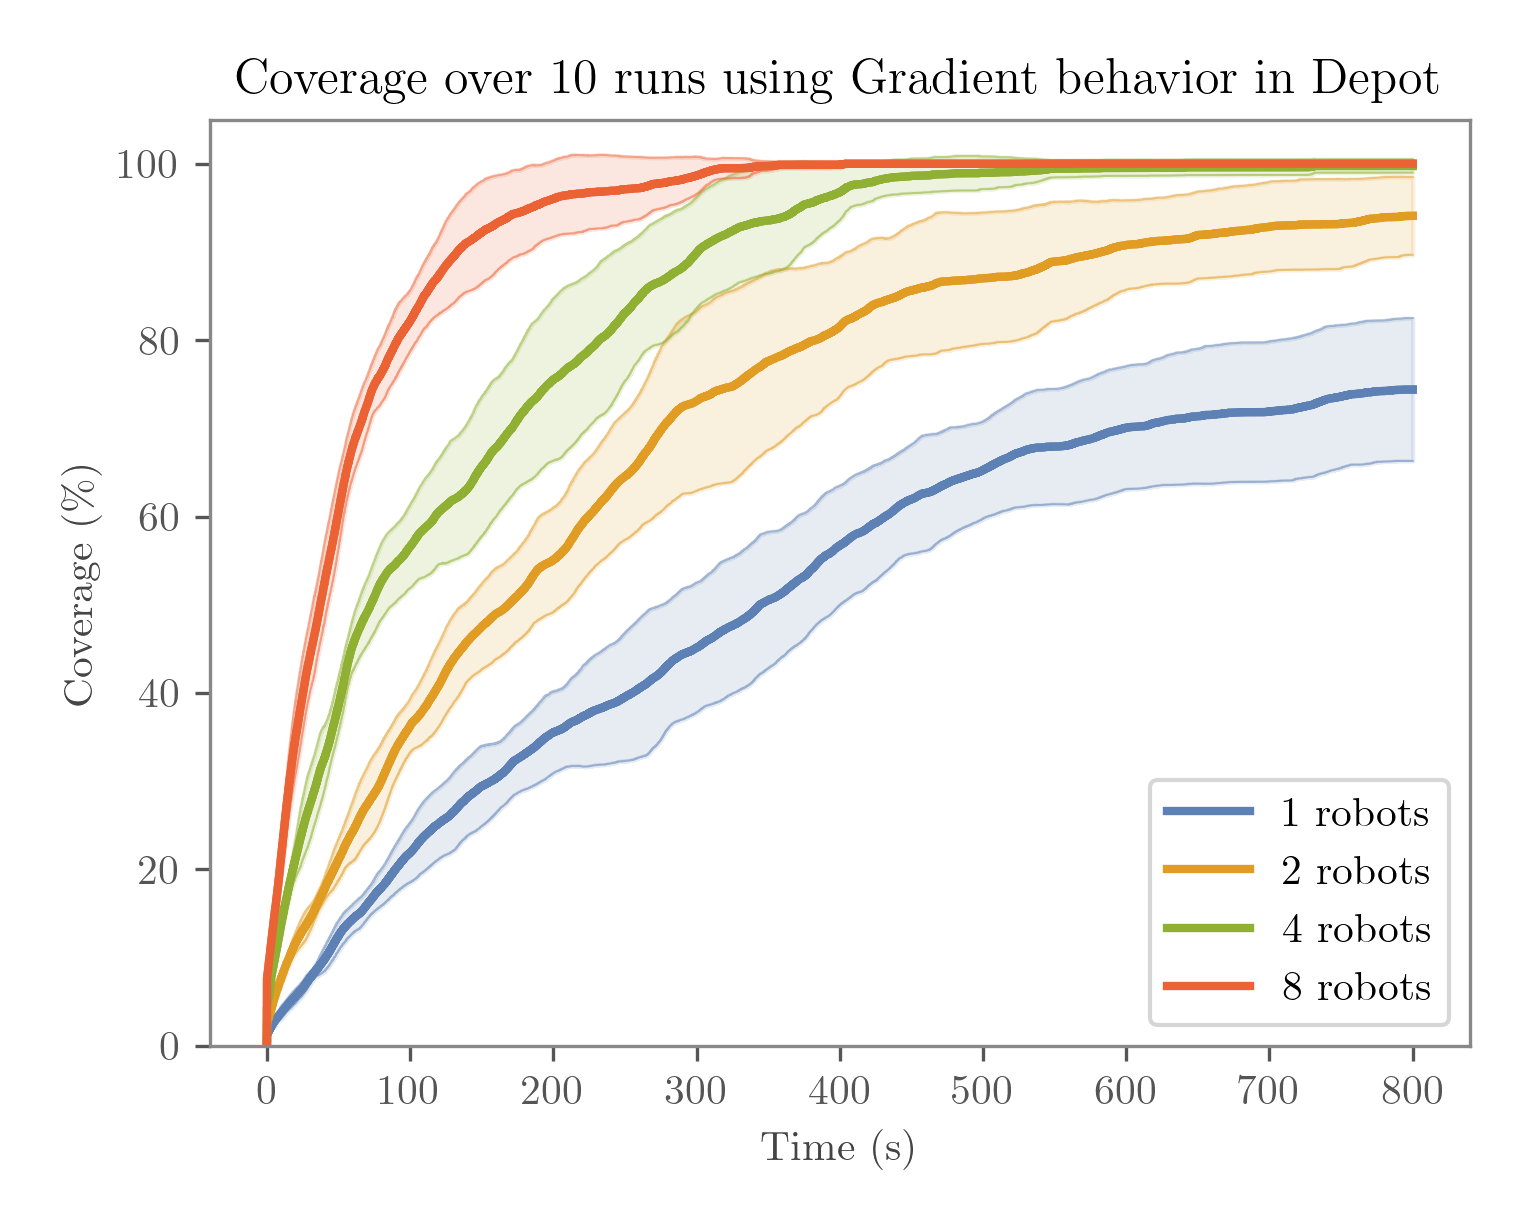
\includegraphics[width=\w]{figures/plots/benchmarks/coverage-over-10-runs-using-gradient-behavior-in-depot.png}
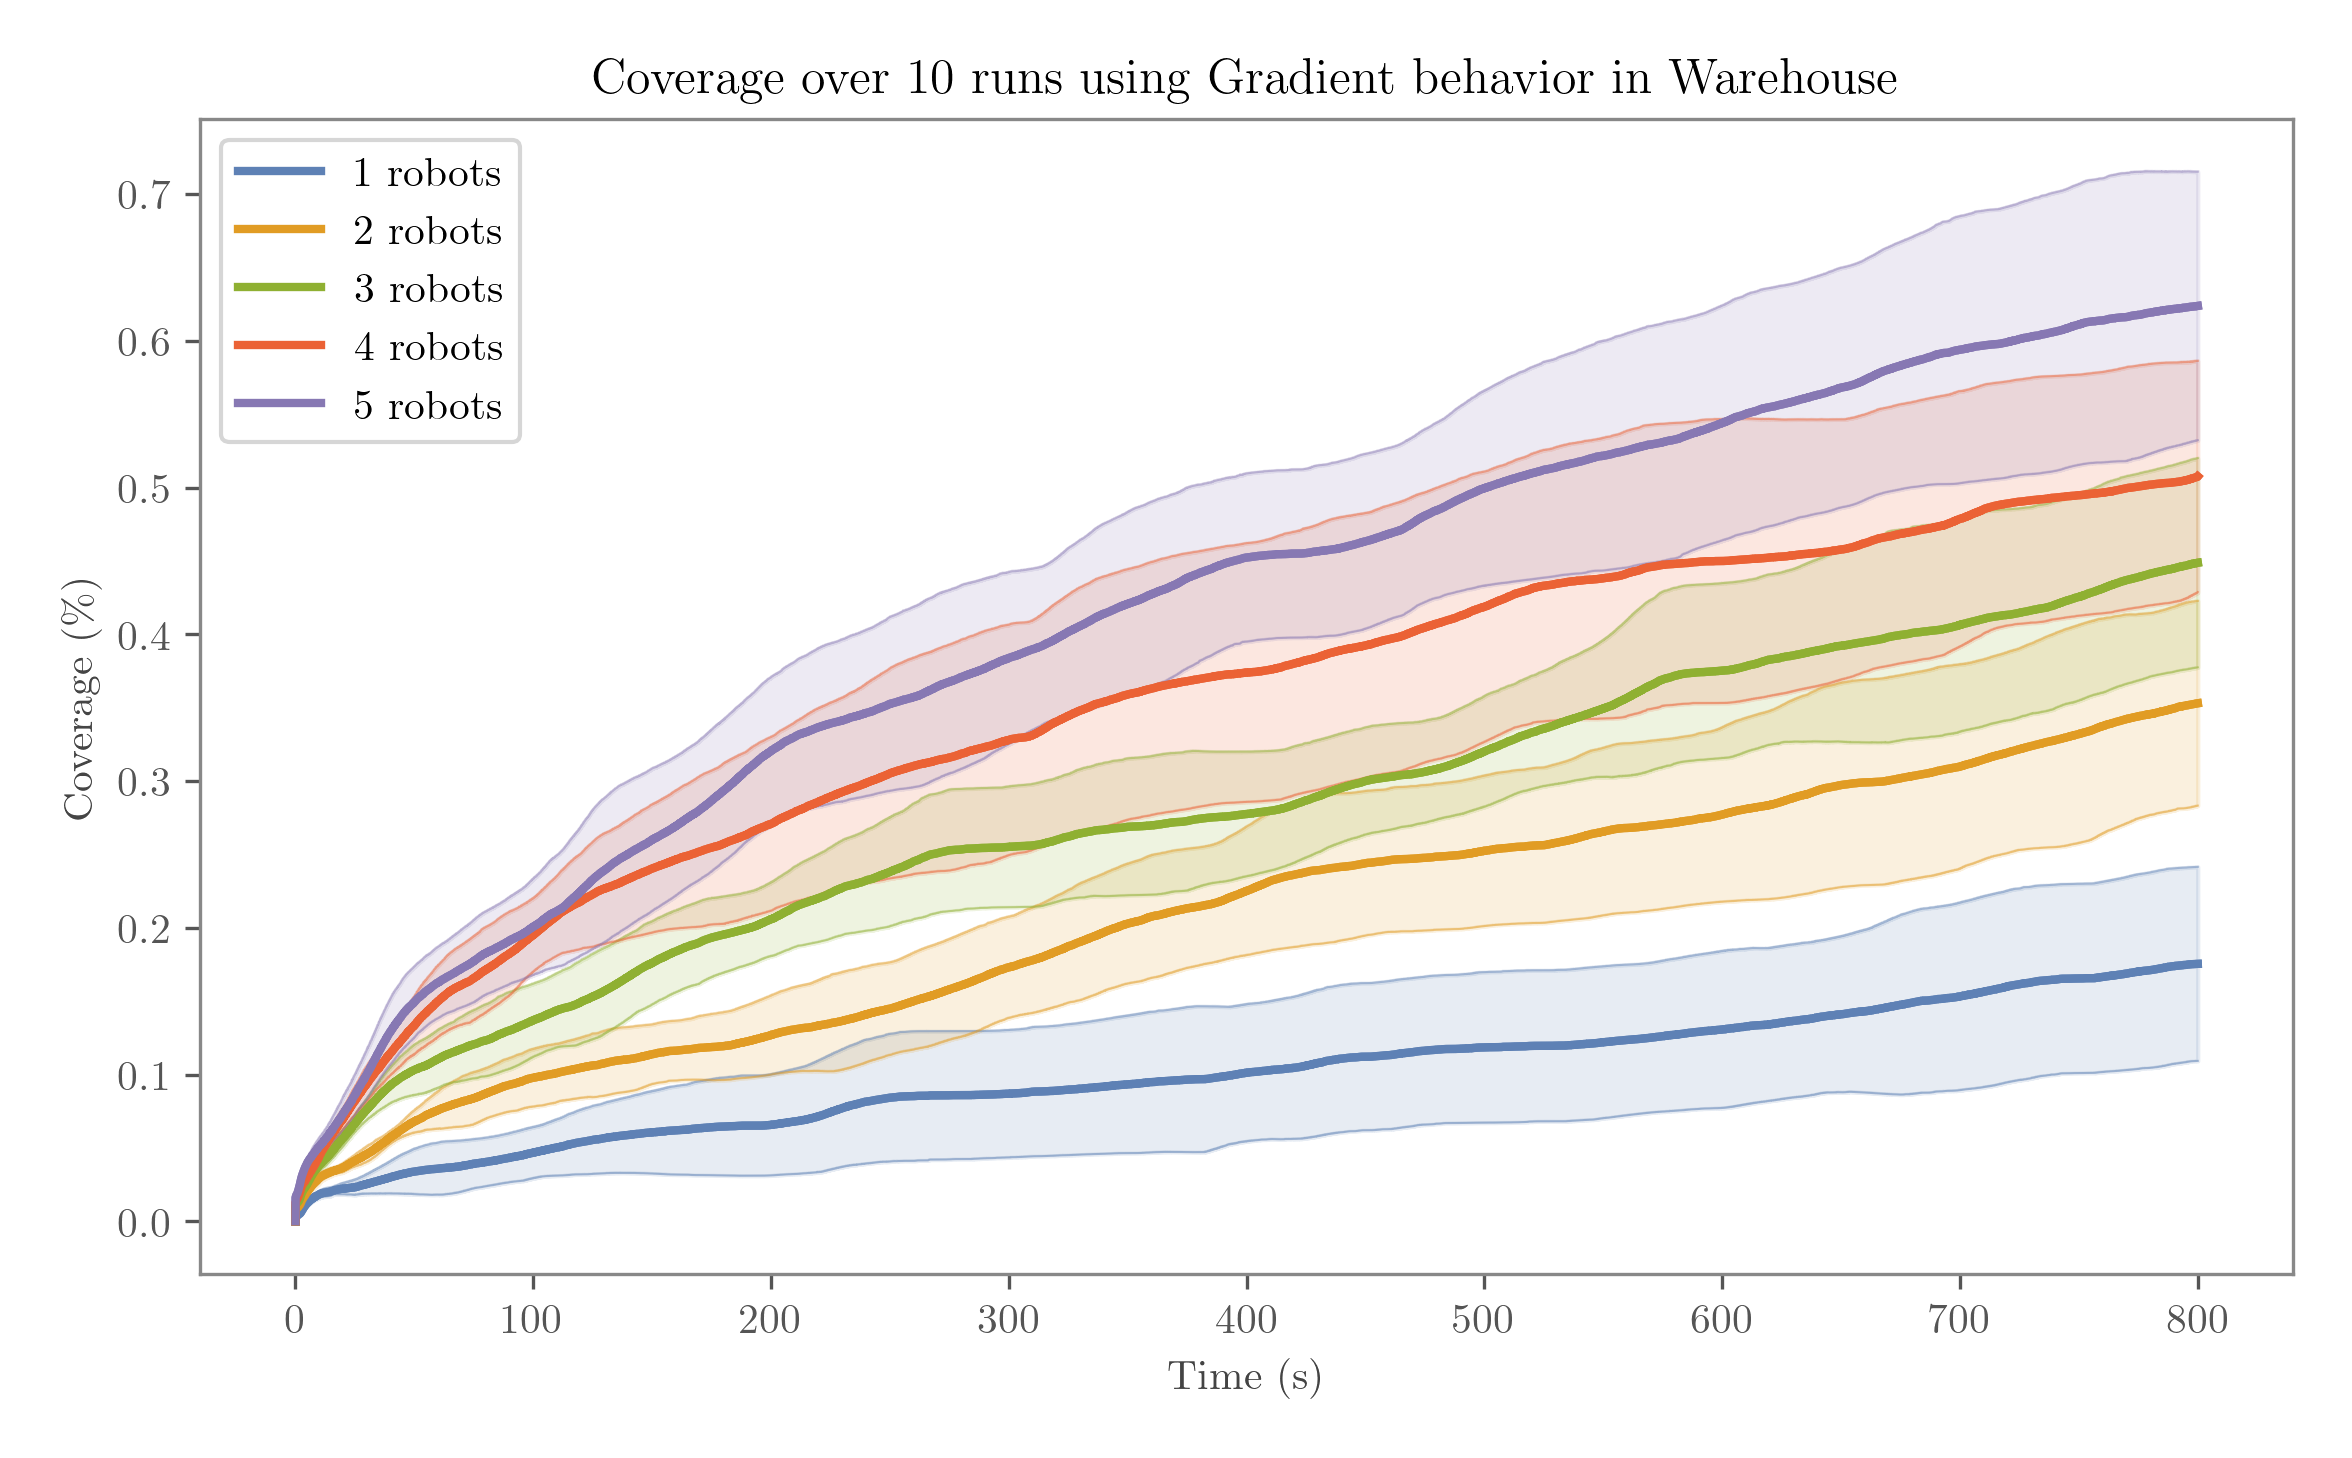
\includegraphics[width=\w]{figures/plots/benchmarks/coverage-over-10-runs-using-gradient-behavior-in-warehouse.png}
\\
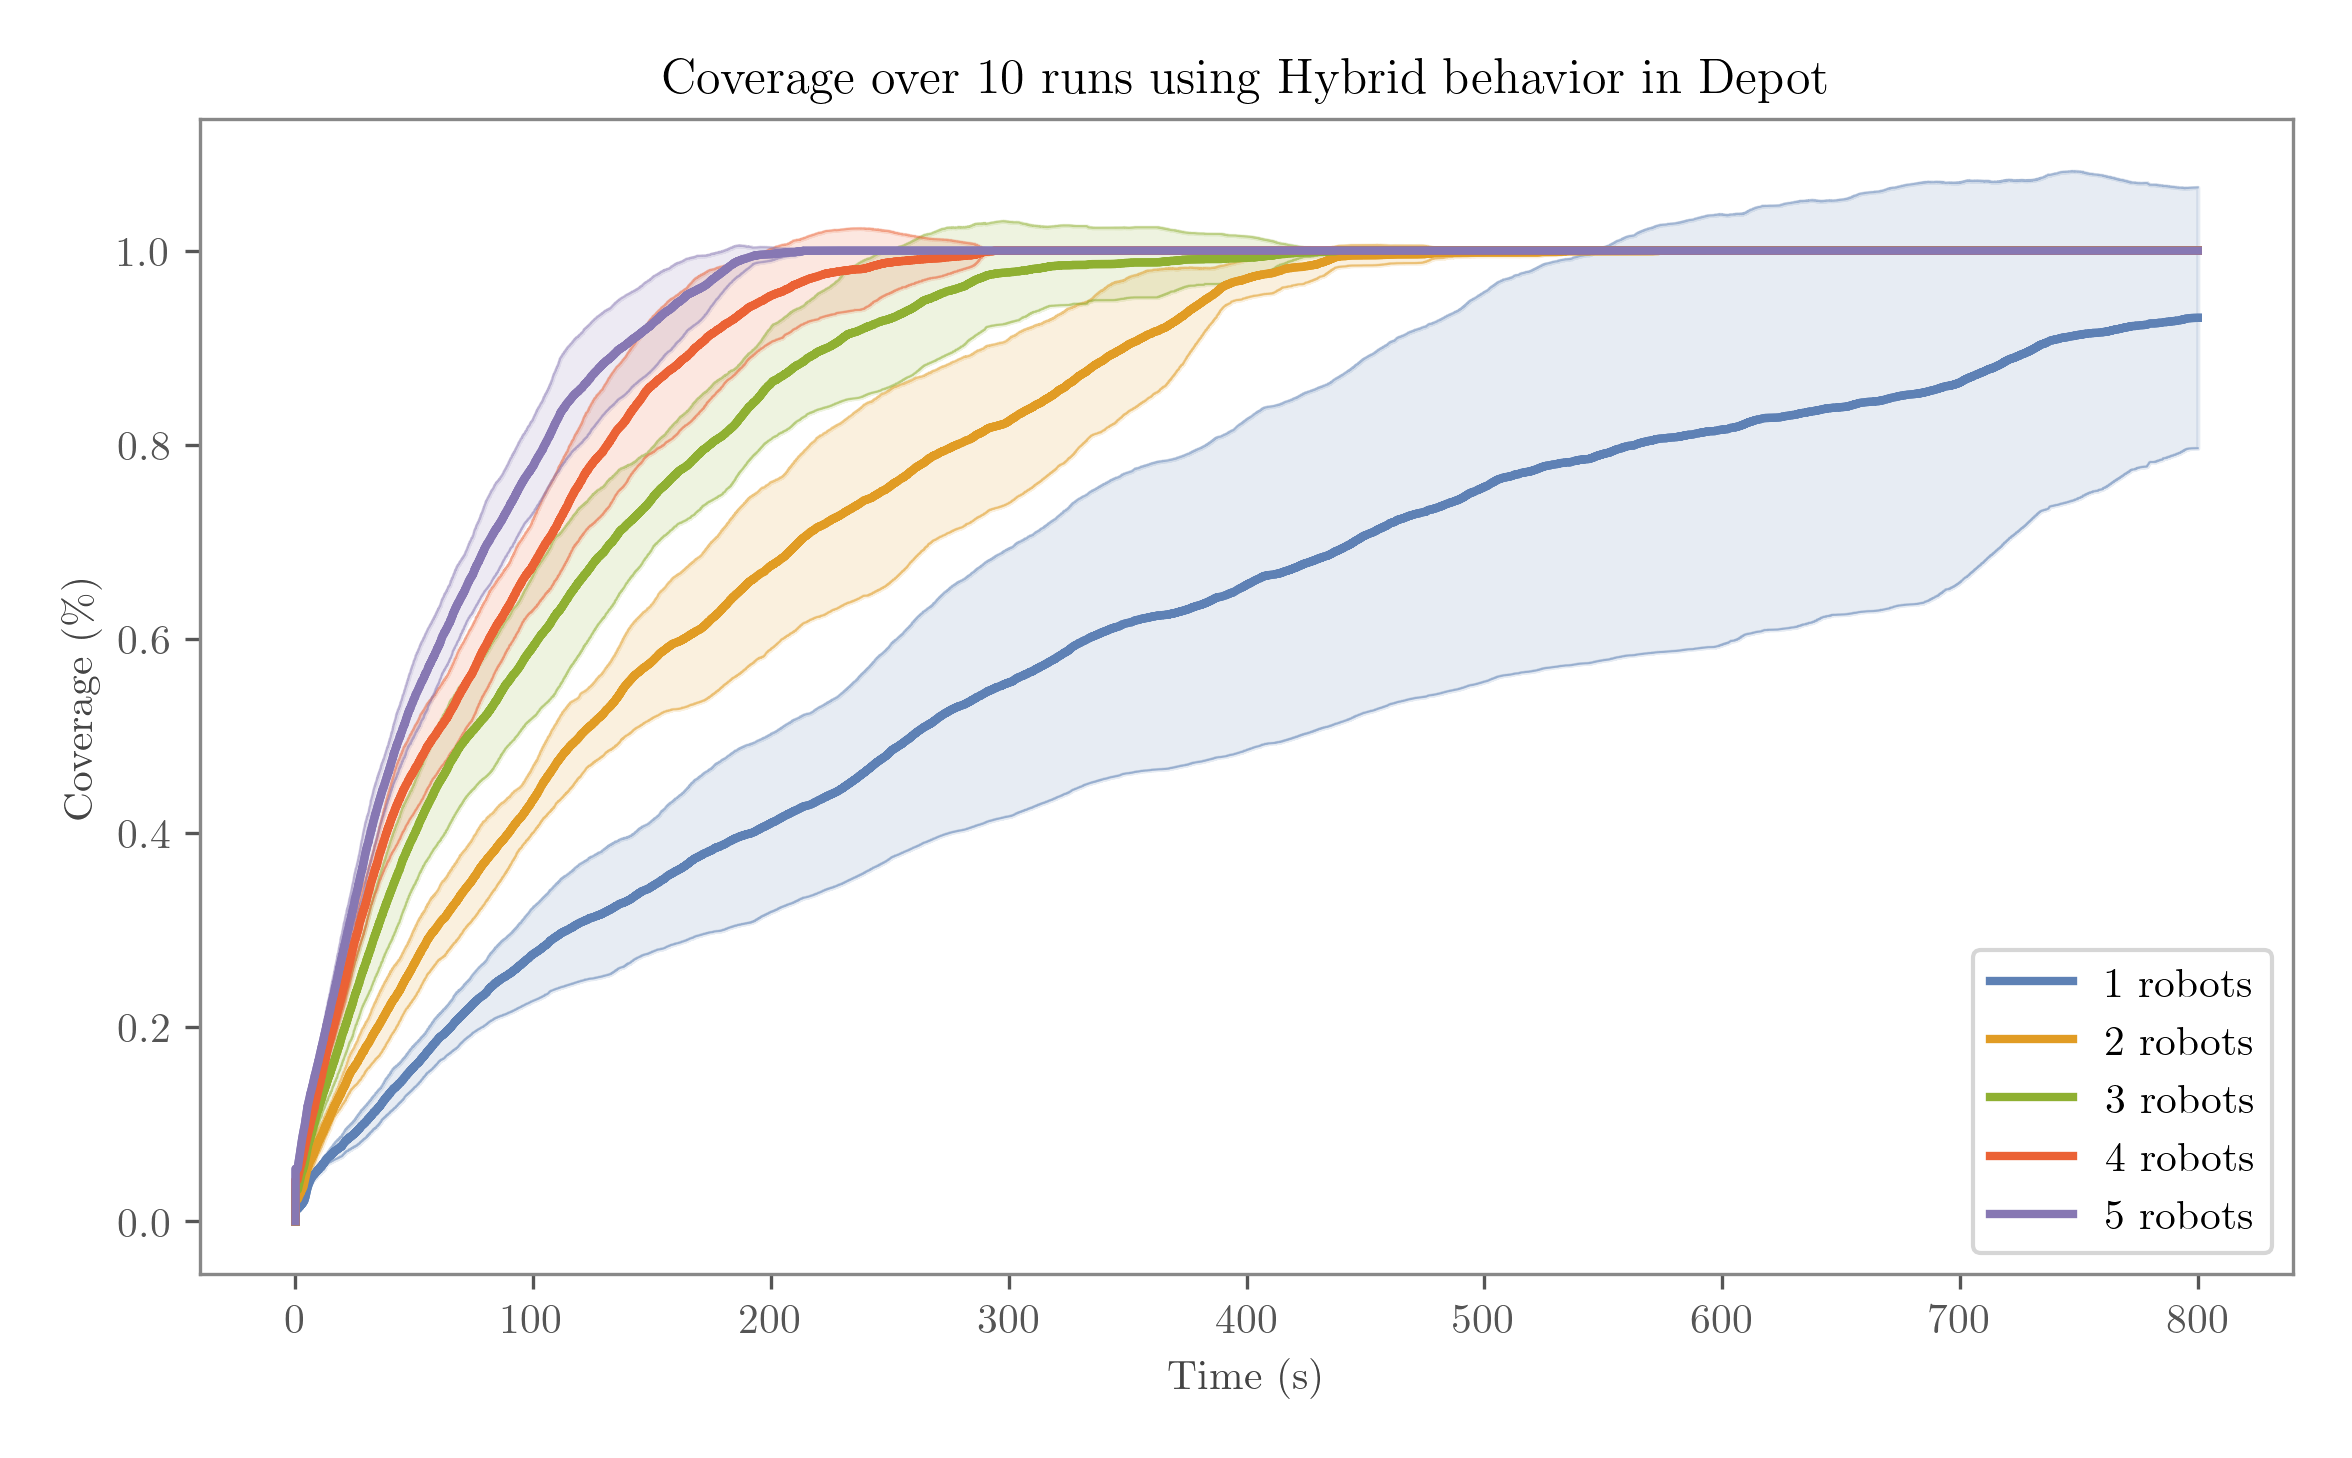
\includegraphics[width=\w]{figures/plots/benchmarks/coverage-over-10-runs-using-hybrid-behavior-in-depot.png}
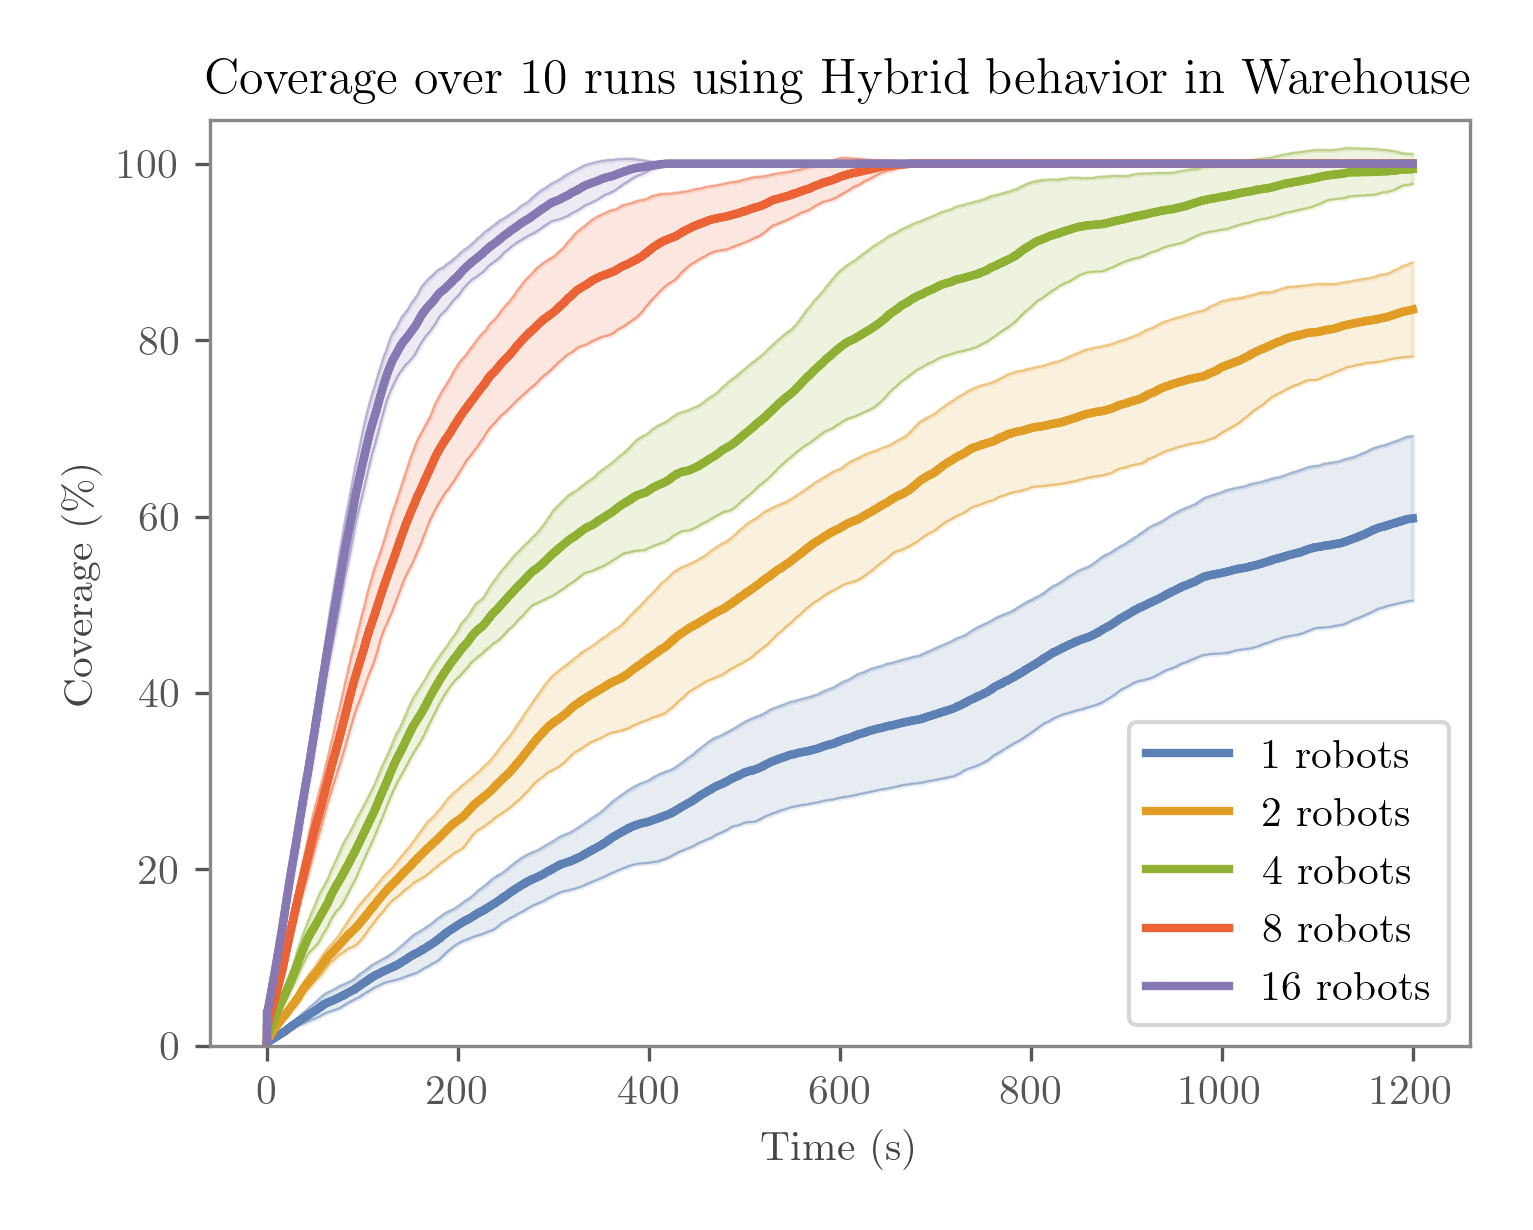
\includegraphics[width=\w]{figures/plots/benchmarks/coverage-over-10-runs-using-hybrid-behavior-in-warehouse.png}
\\
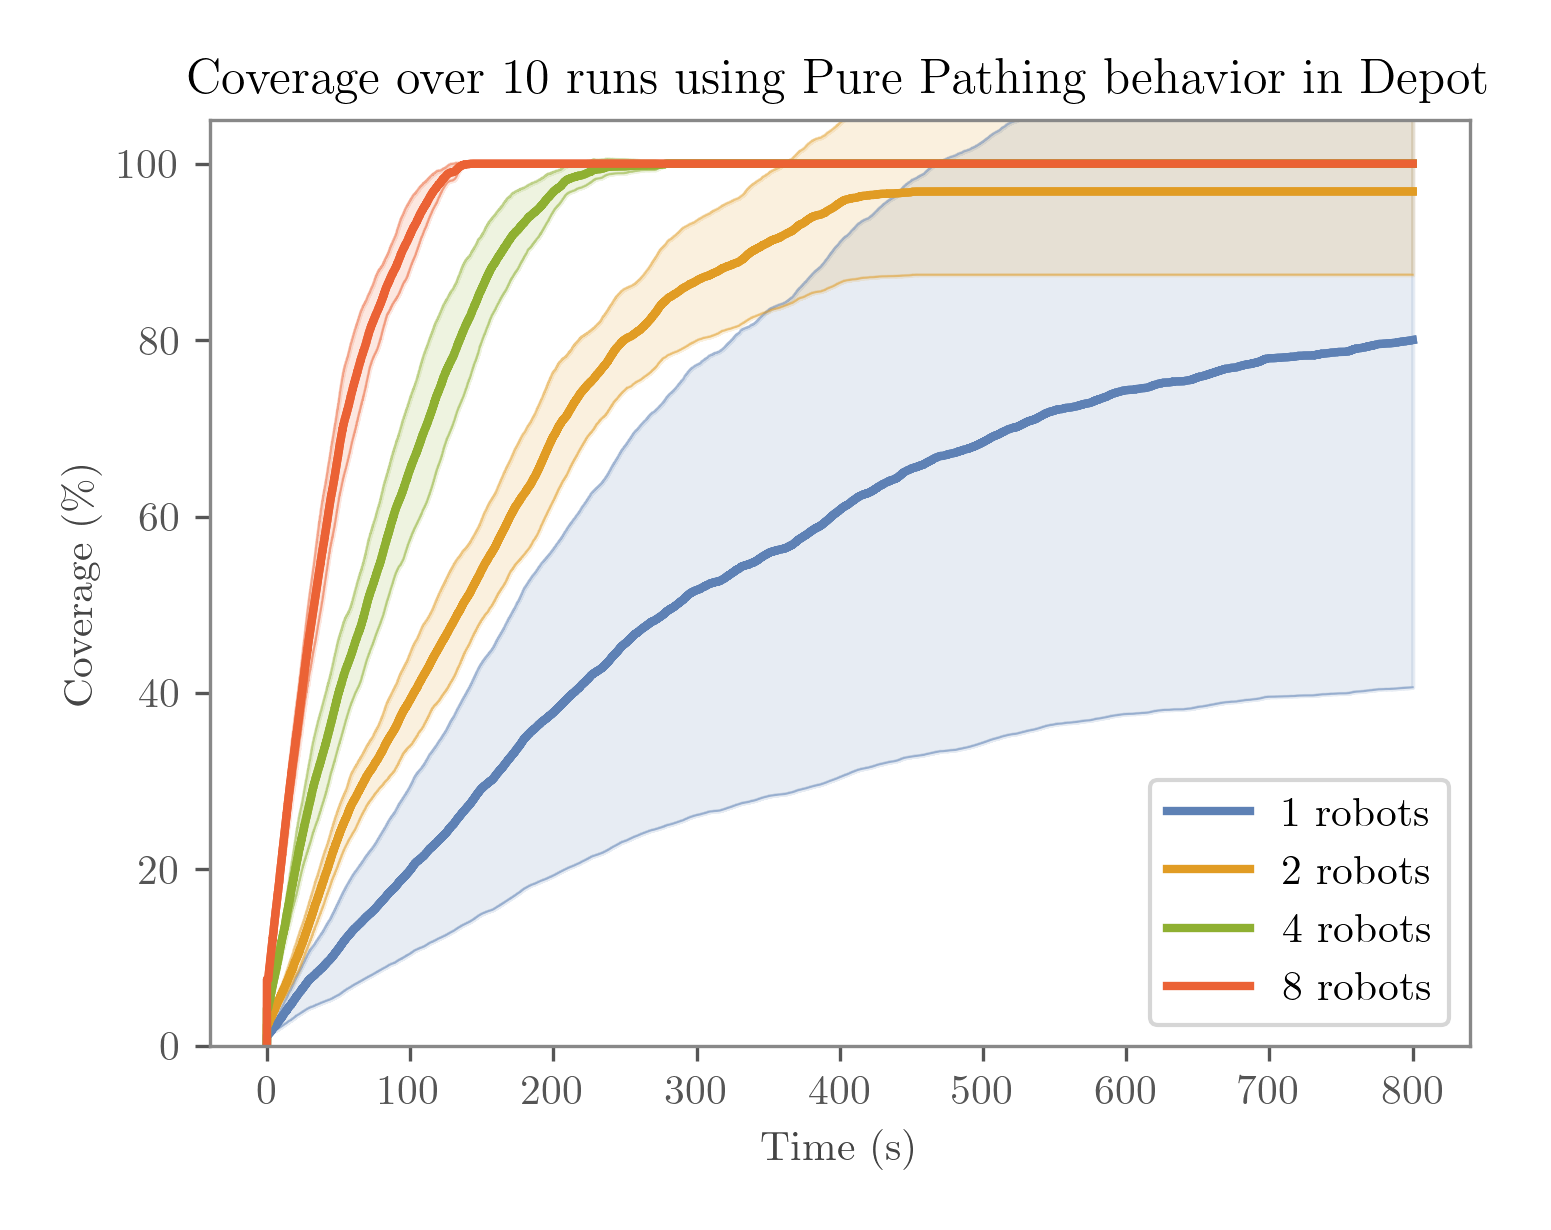
\includegraphics[width=\w]{figures/plots/benchmarks/coverage-over-10-runs-using-pure-pathing-behavior-in-depot.png}
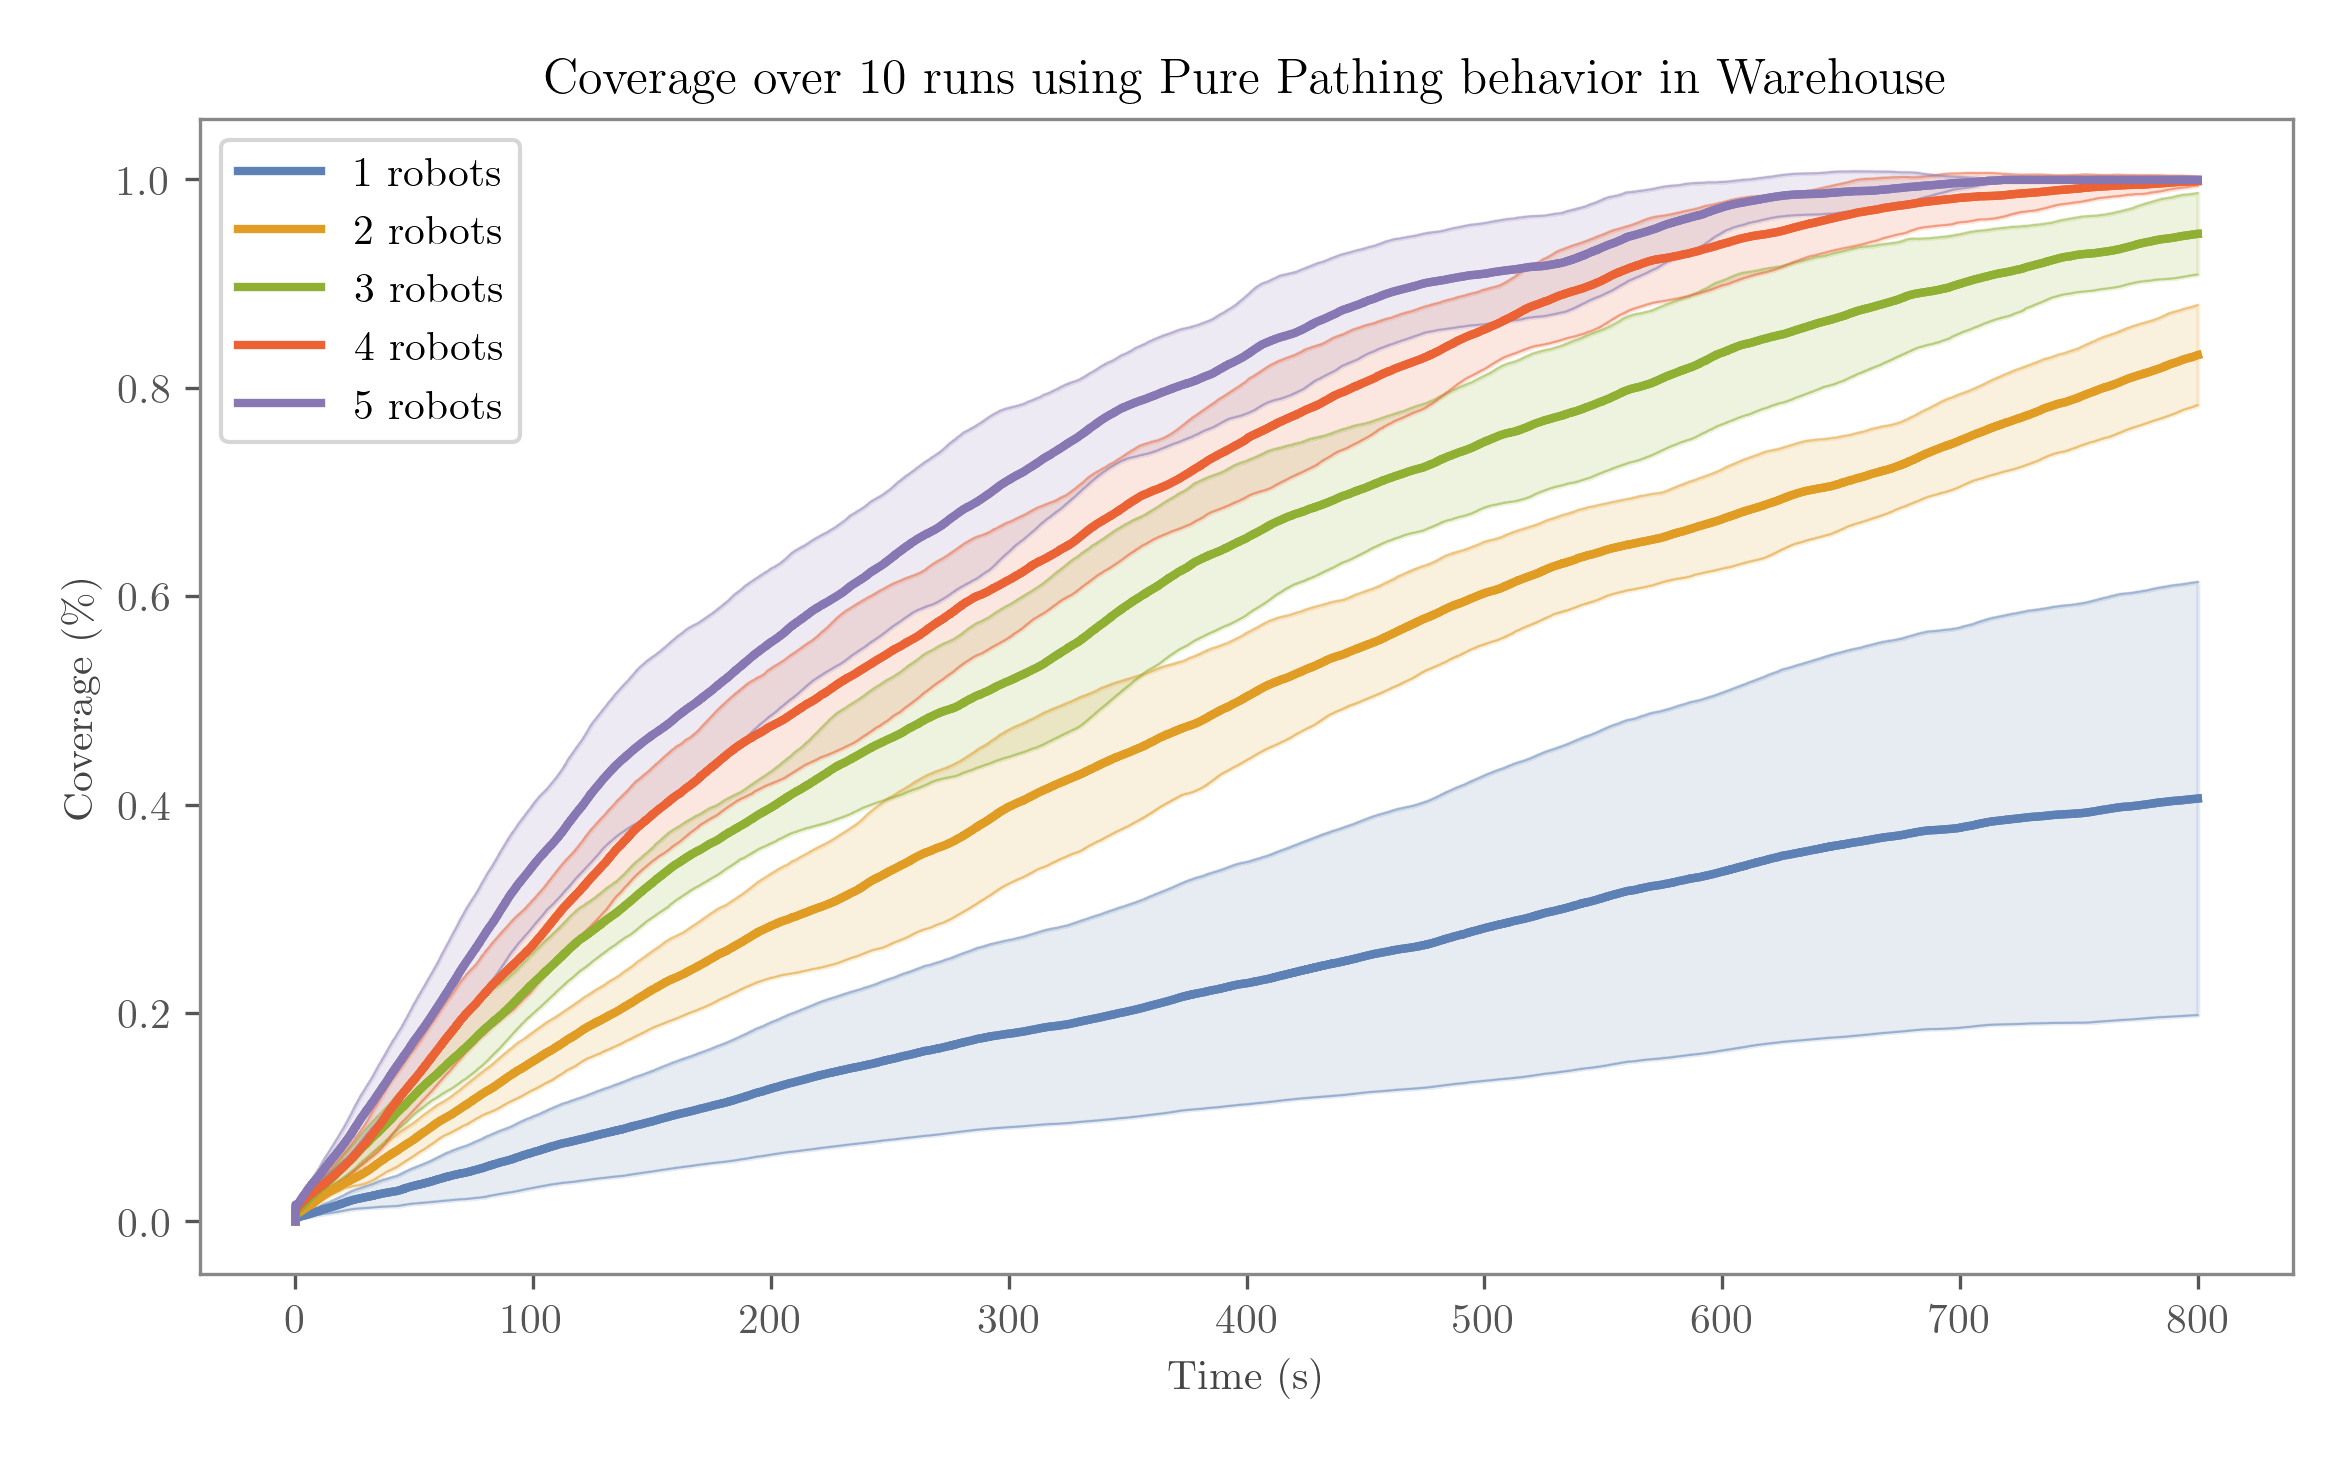
\includegraphics[width=\w]{figures/plots/benchmarks/coverage-over-10-runs-using-pure-pathing-behavior-in-warehouse.png}
\\
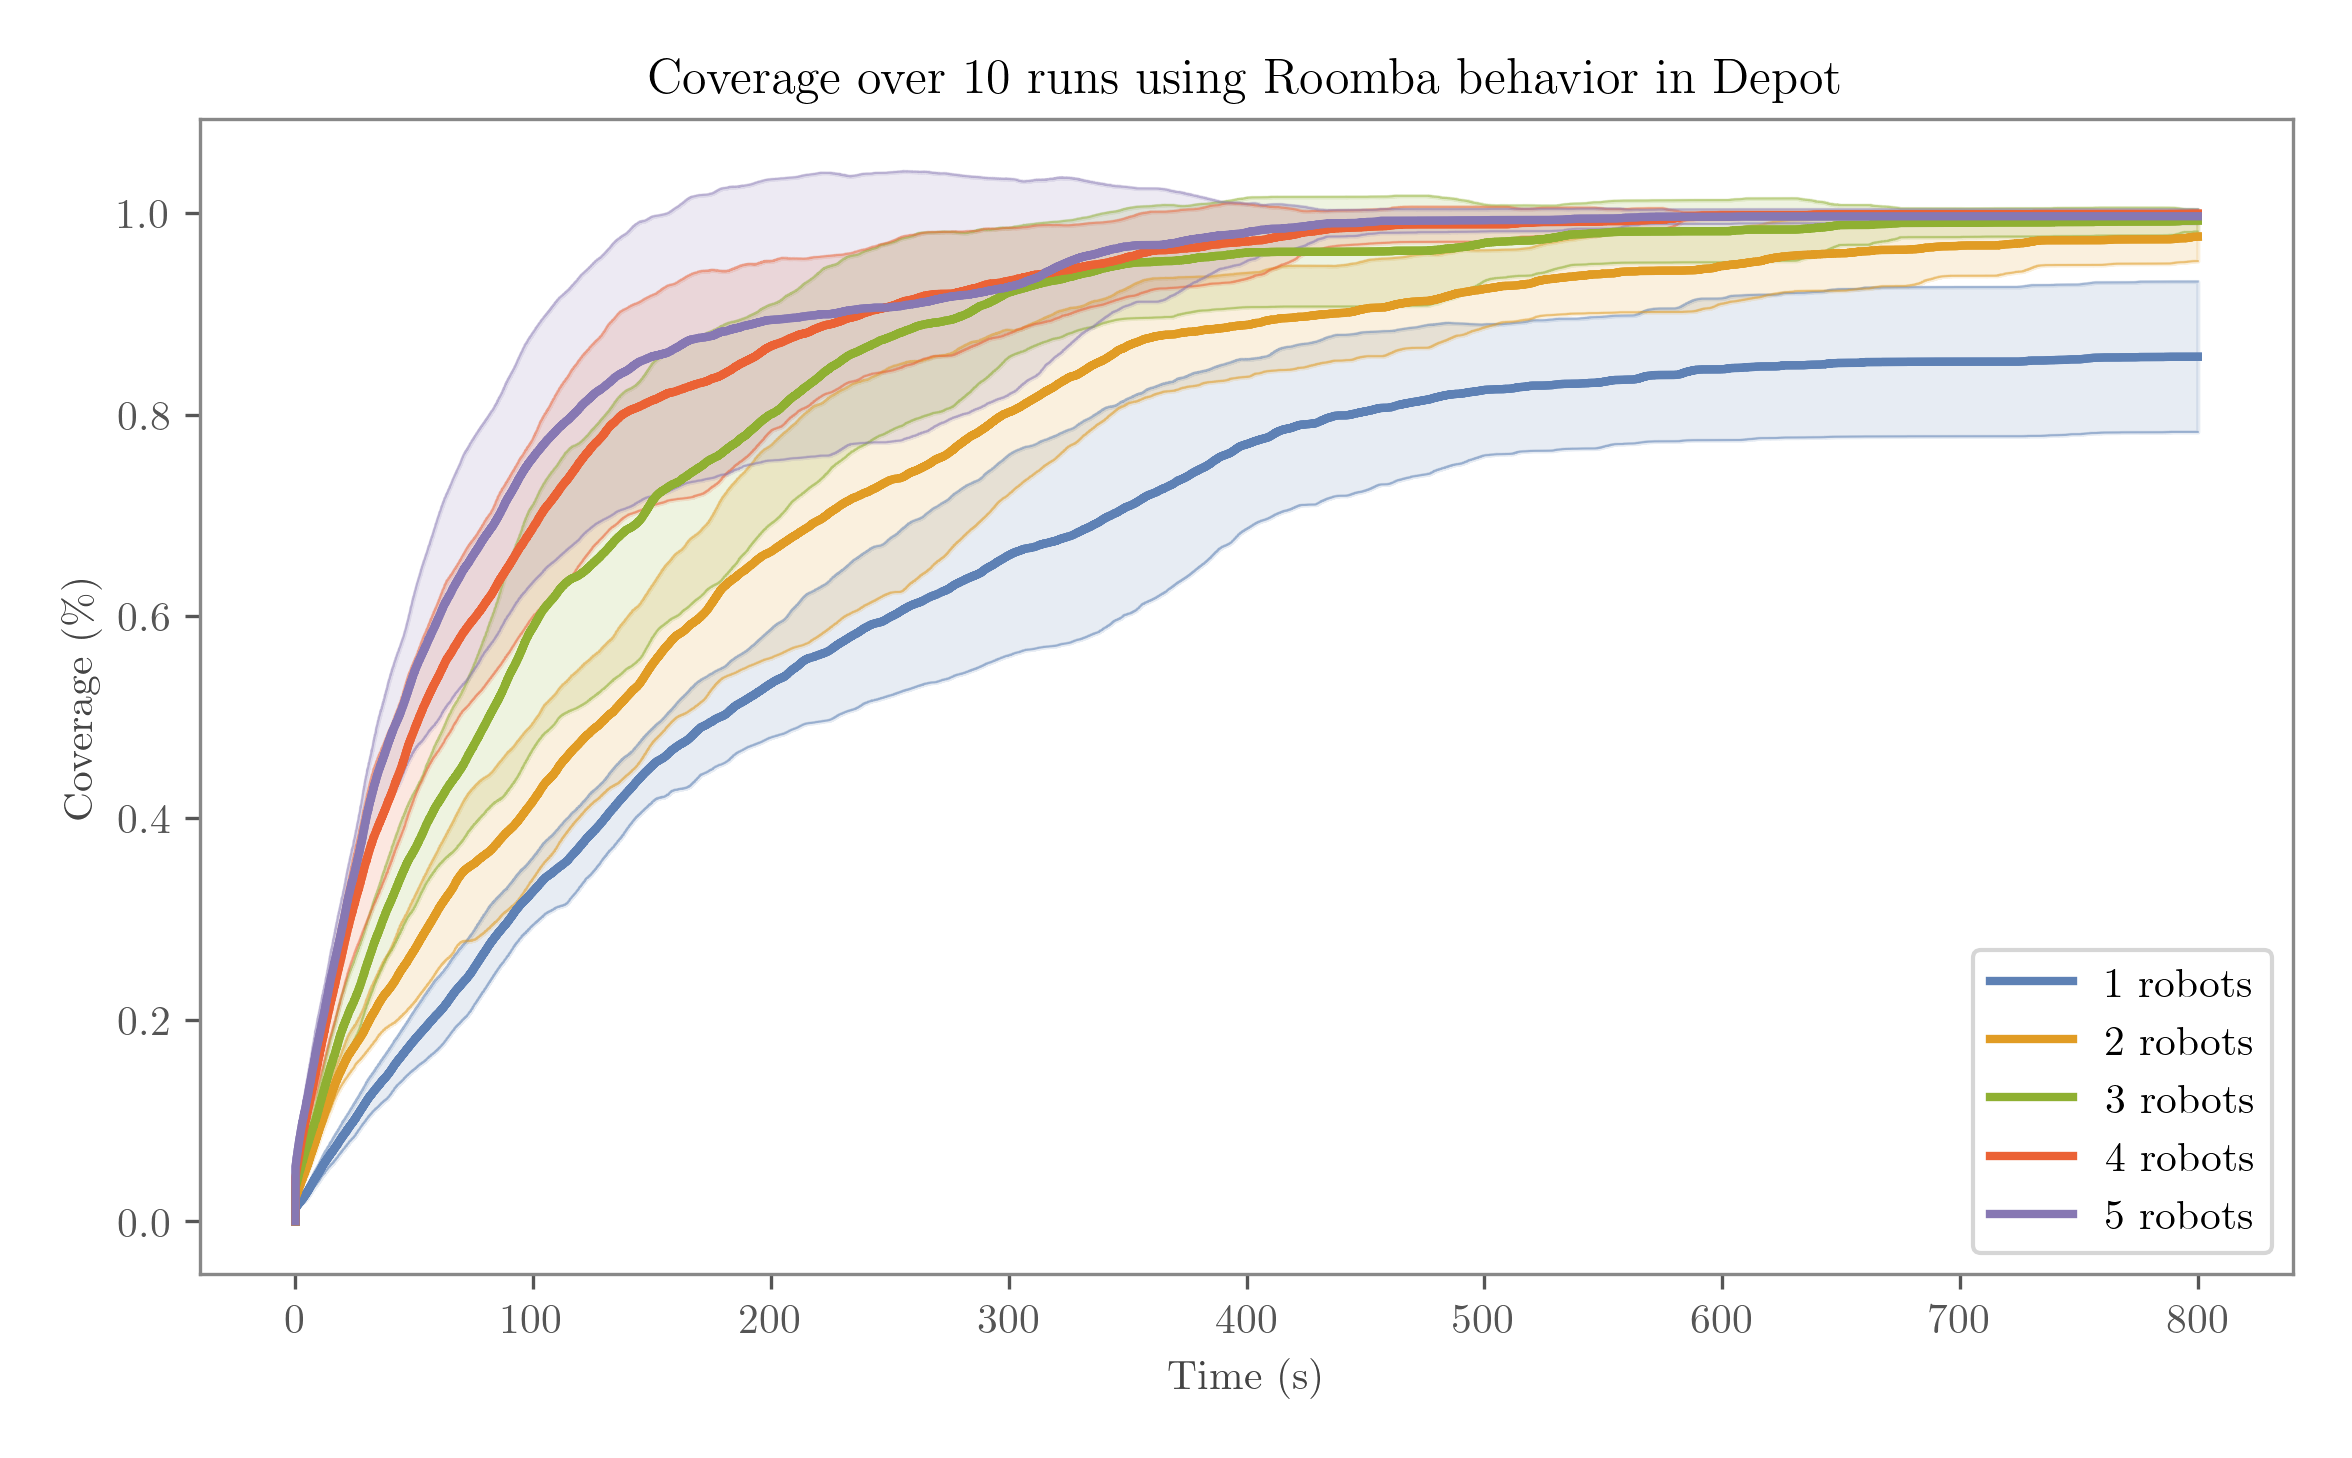
\includegraphics[width=\w]{figures/plots/benchmarks/coverage-over-10-runs-using-roomba-behavior-in-depot.png}
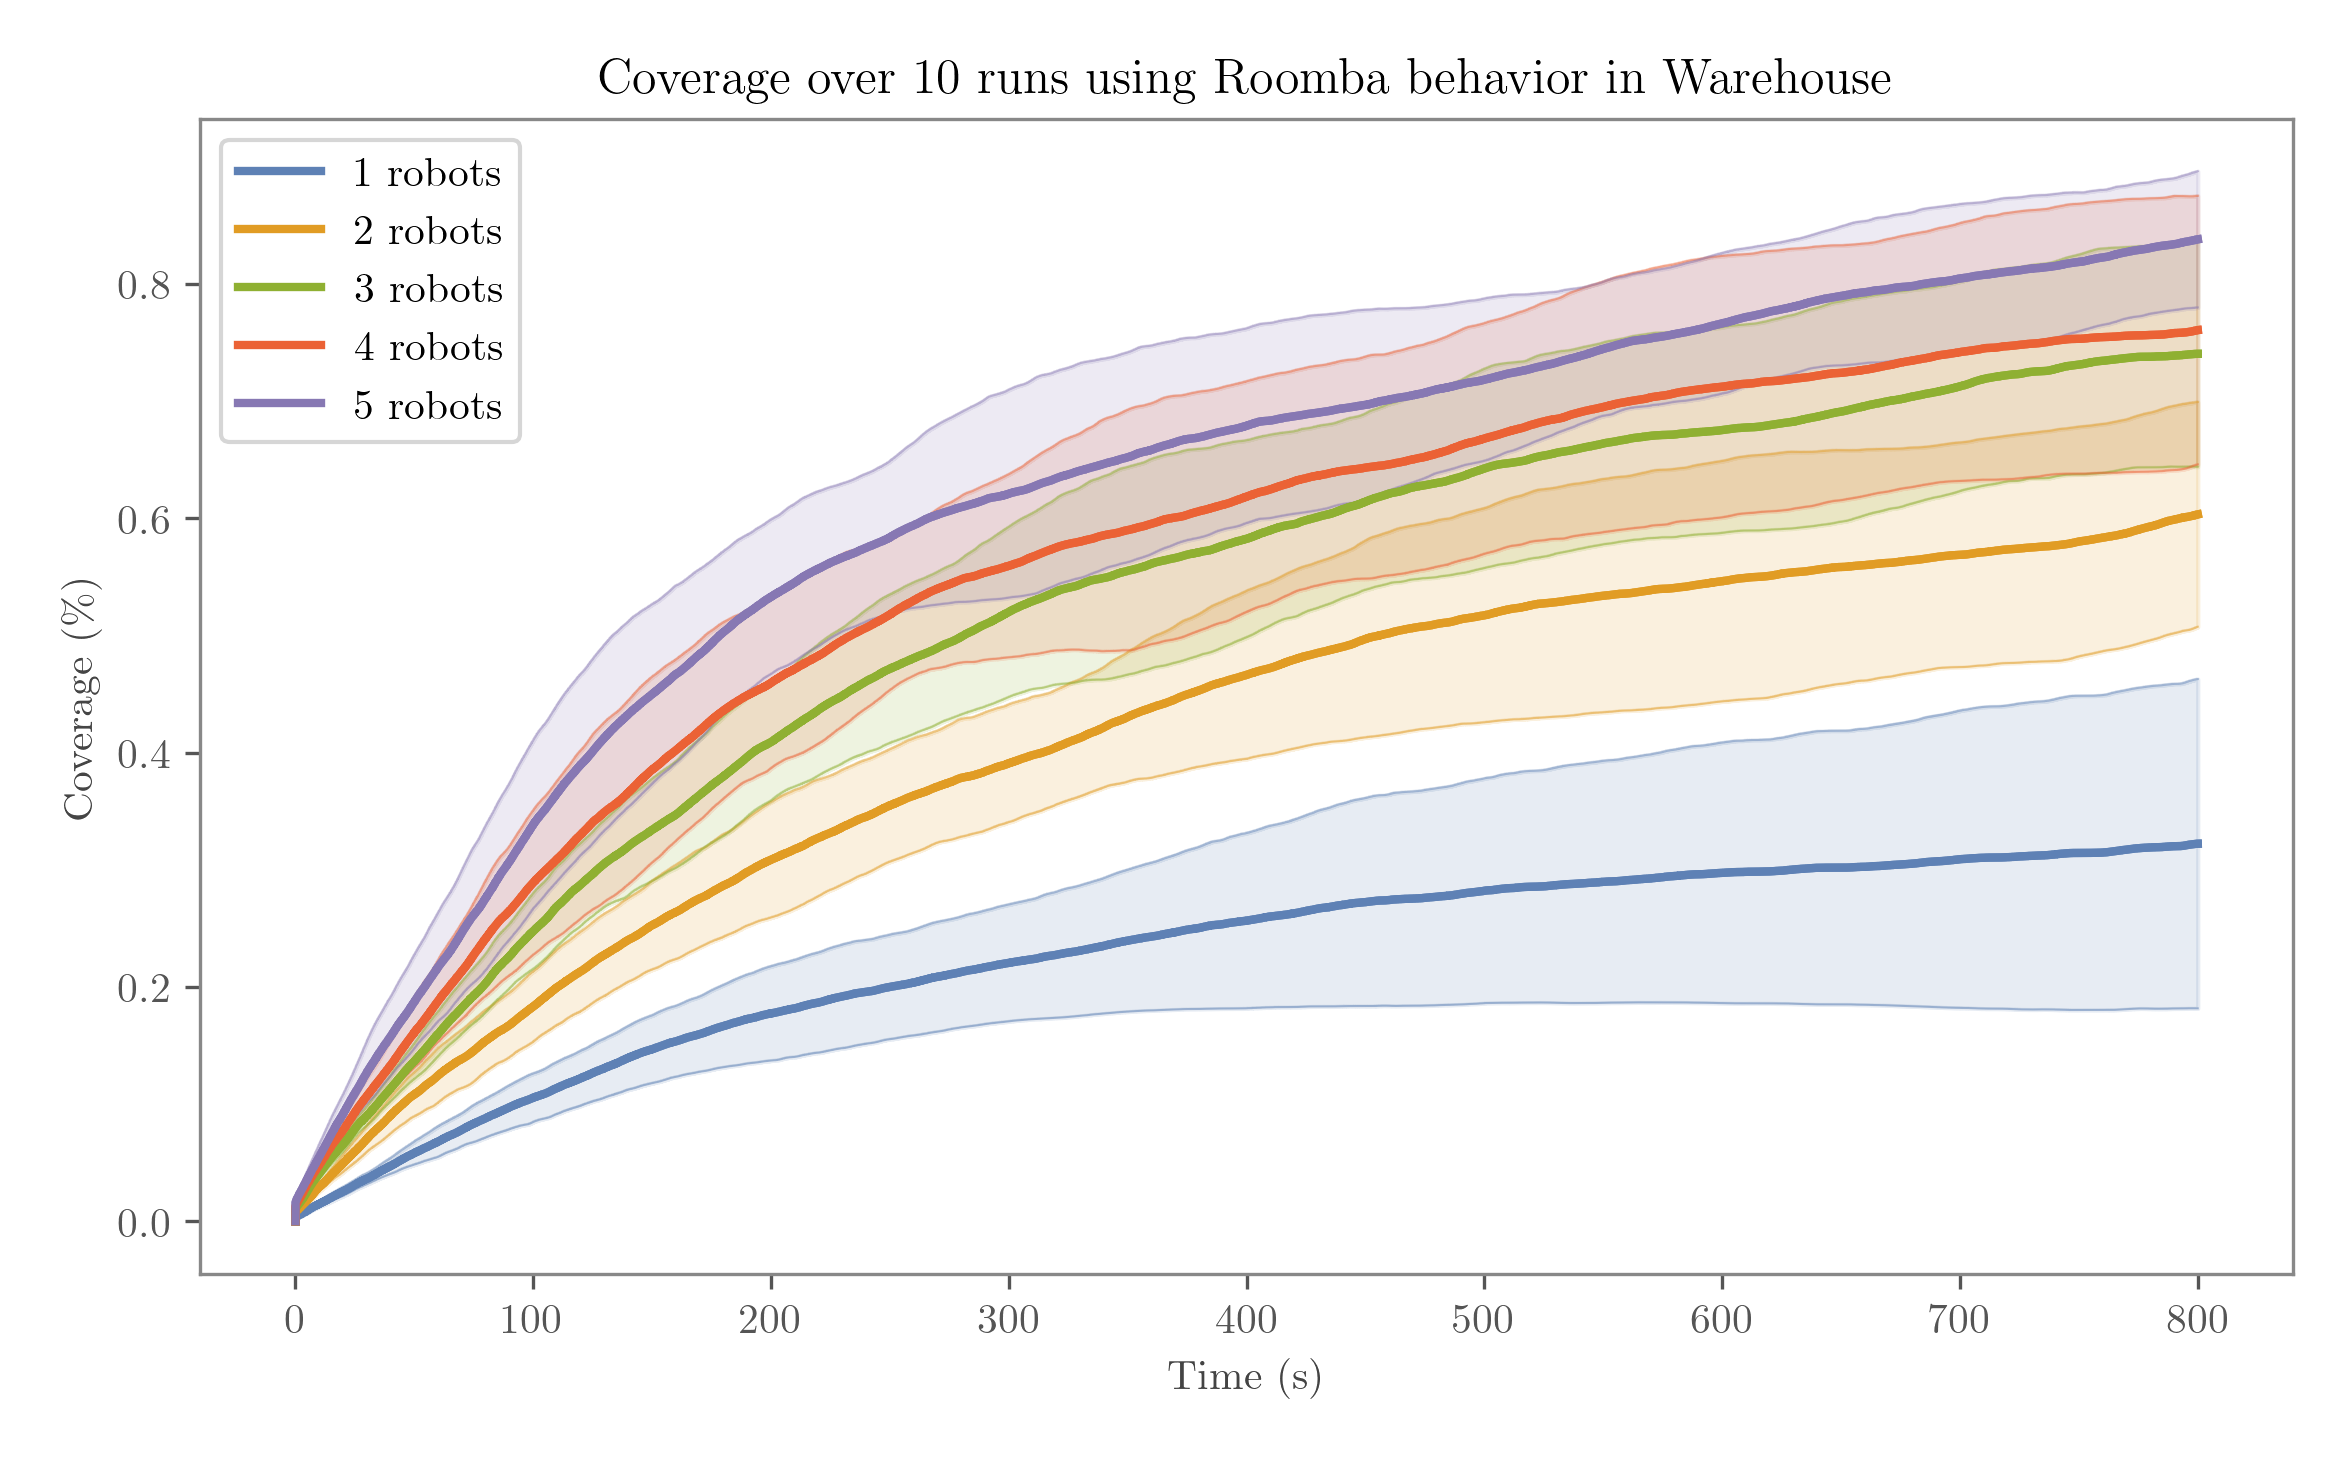
\includegraphics[width=\w]{figures/plots/benchmarks/coverage-over-10-runs-using-roomba-behavior-in-warehouse.png}
\\
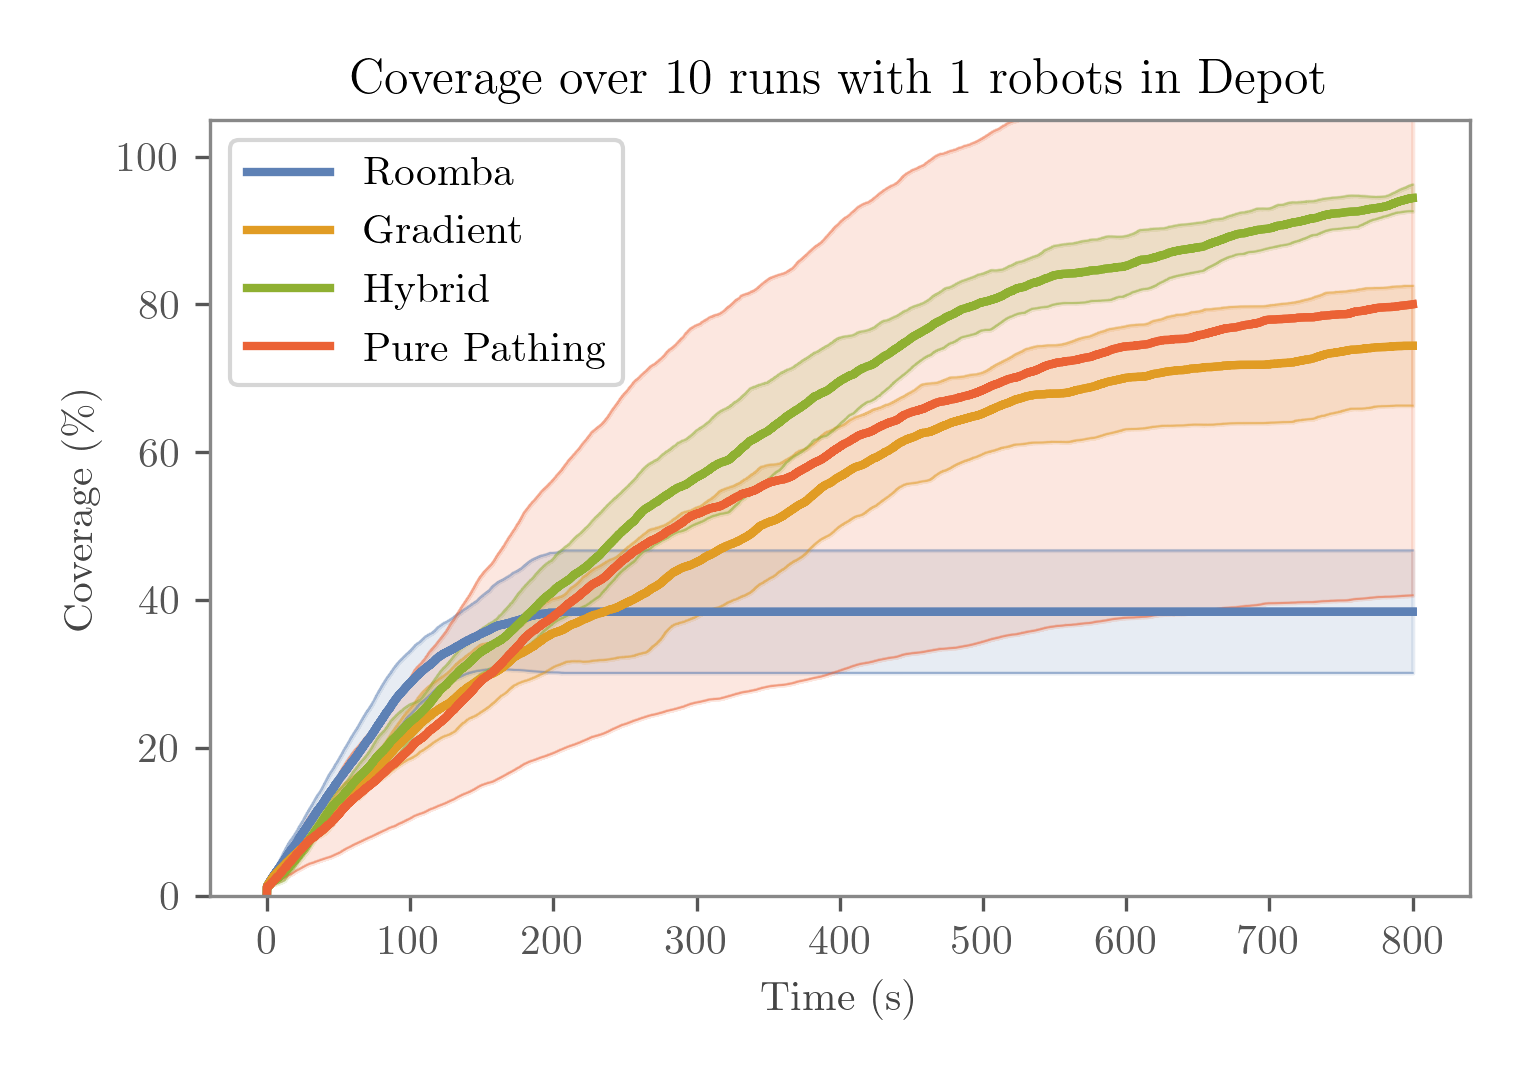
\includegraphics[width=\w]{figures/plots/benchmarks/coverage-over-10-runs-with-1-robots-in-depot.png}
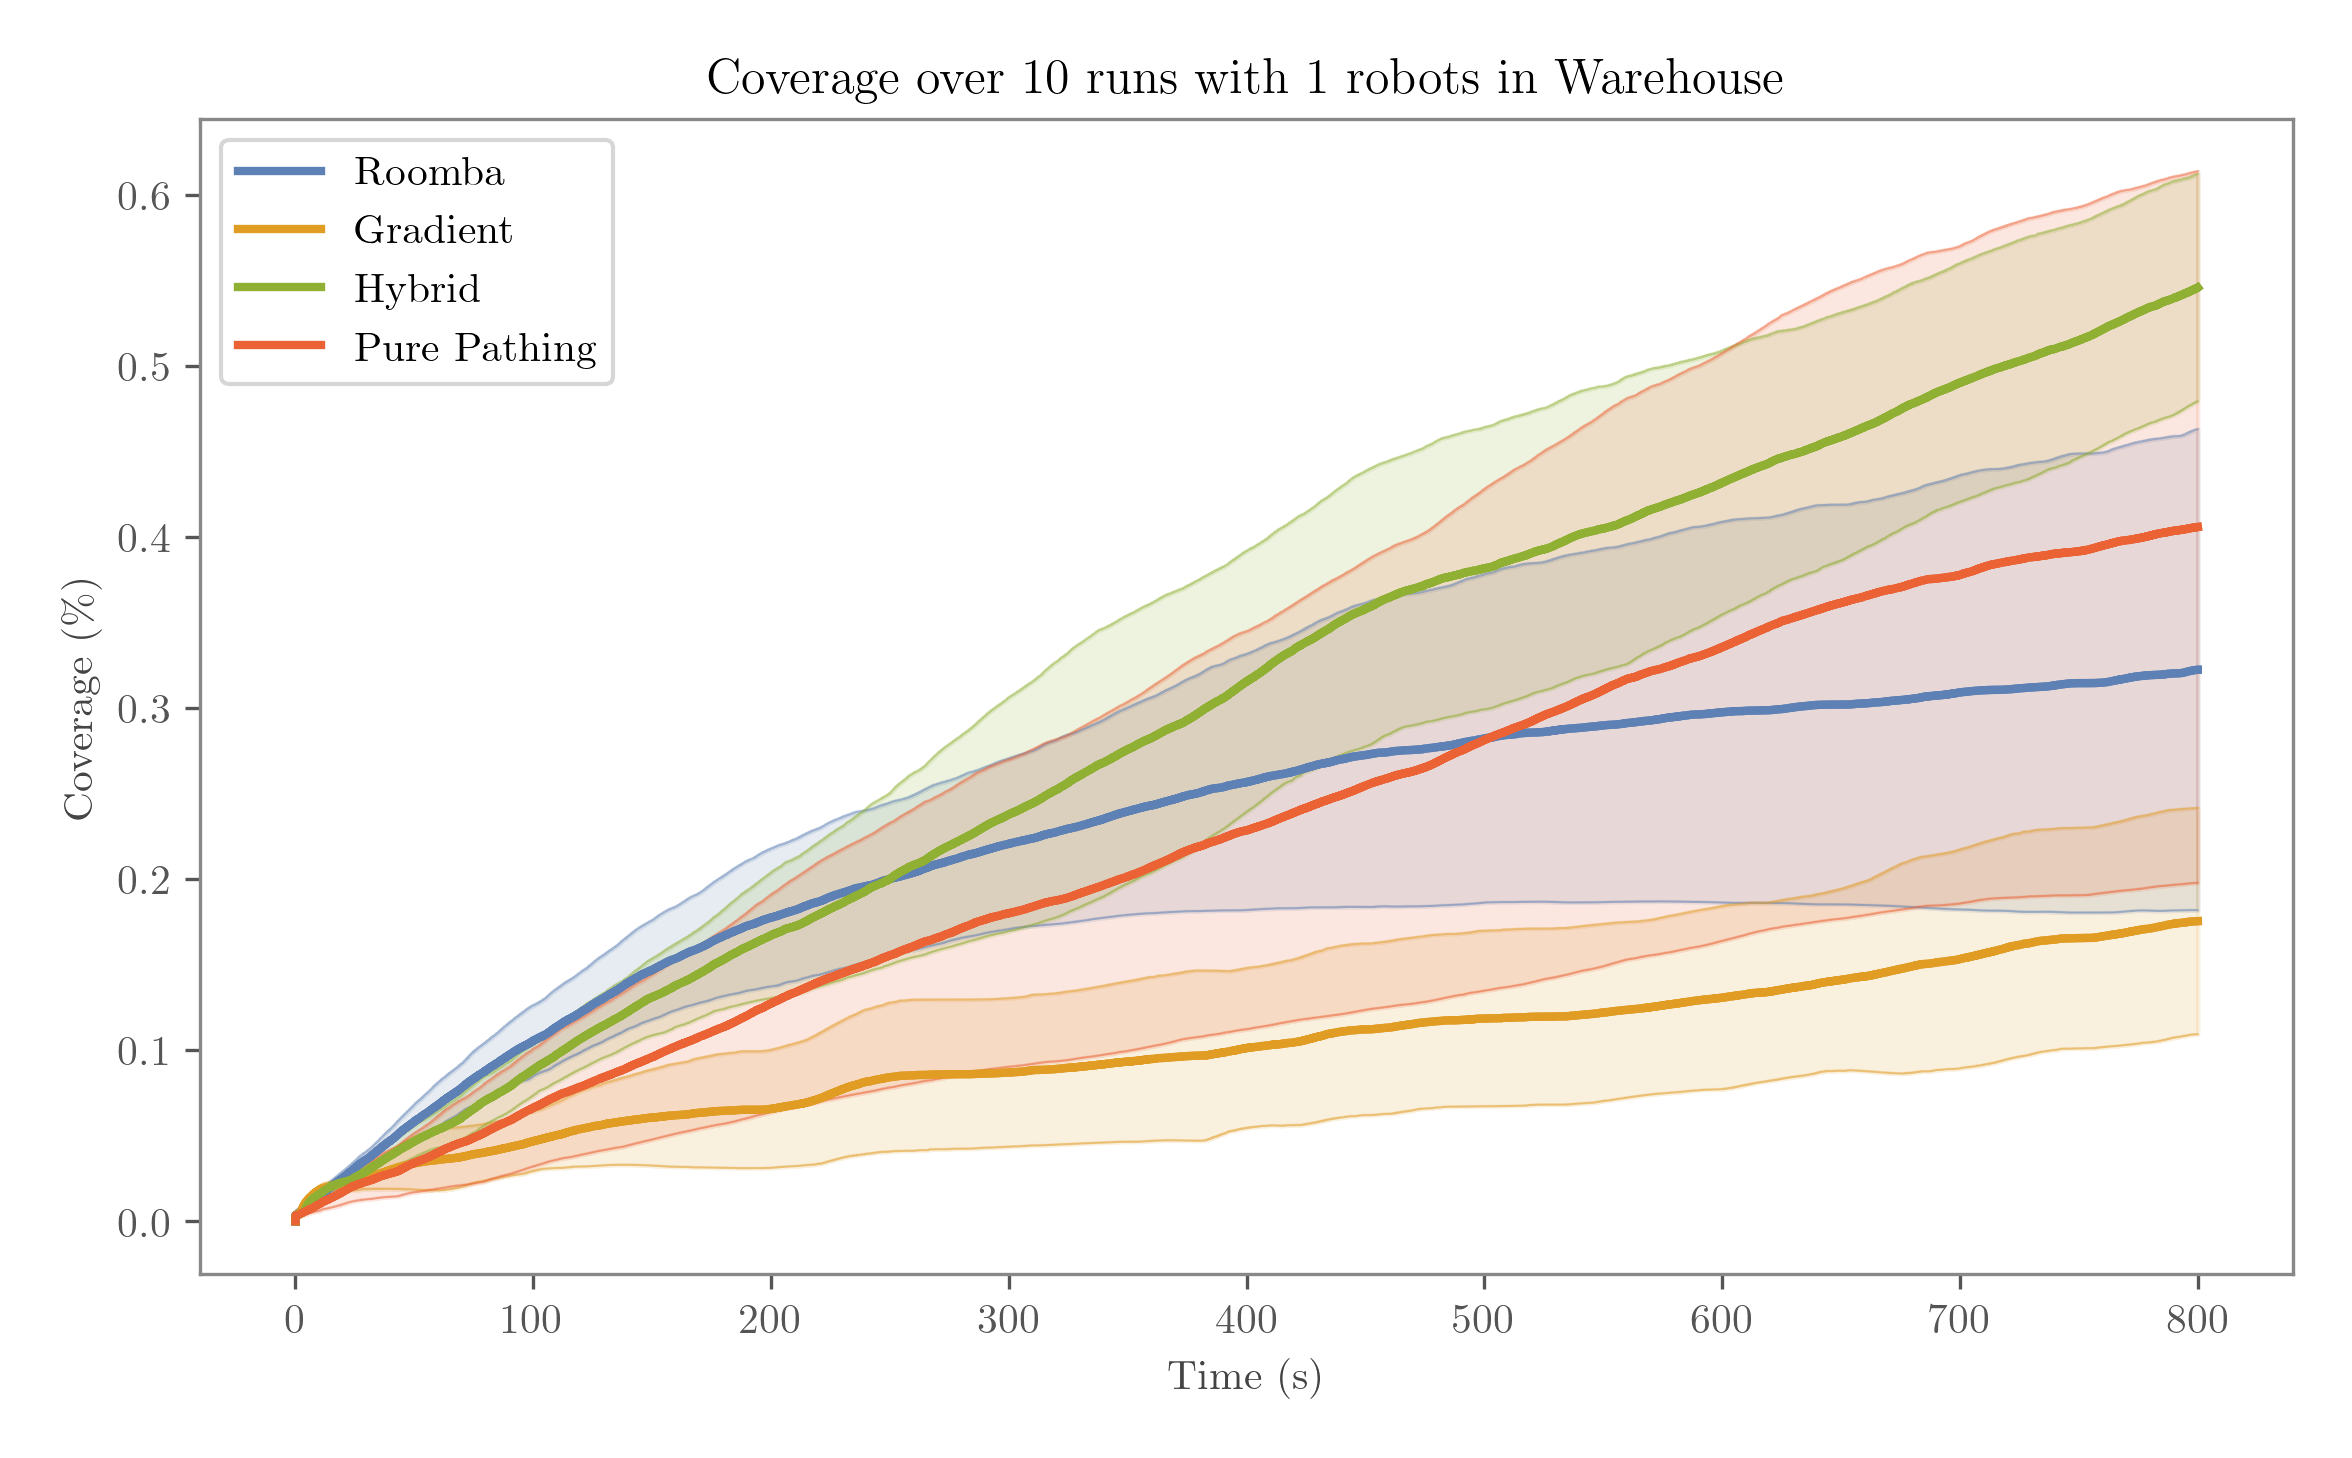
\includegraphics[width=\w]{figures/plots/benchmarks/coverage-over-10-runs-with-1-robots-in-warehouse.png}
\\
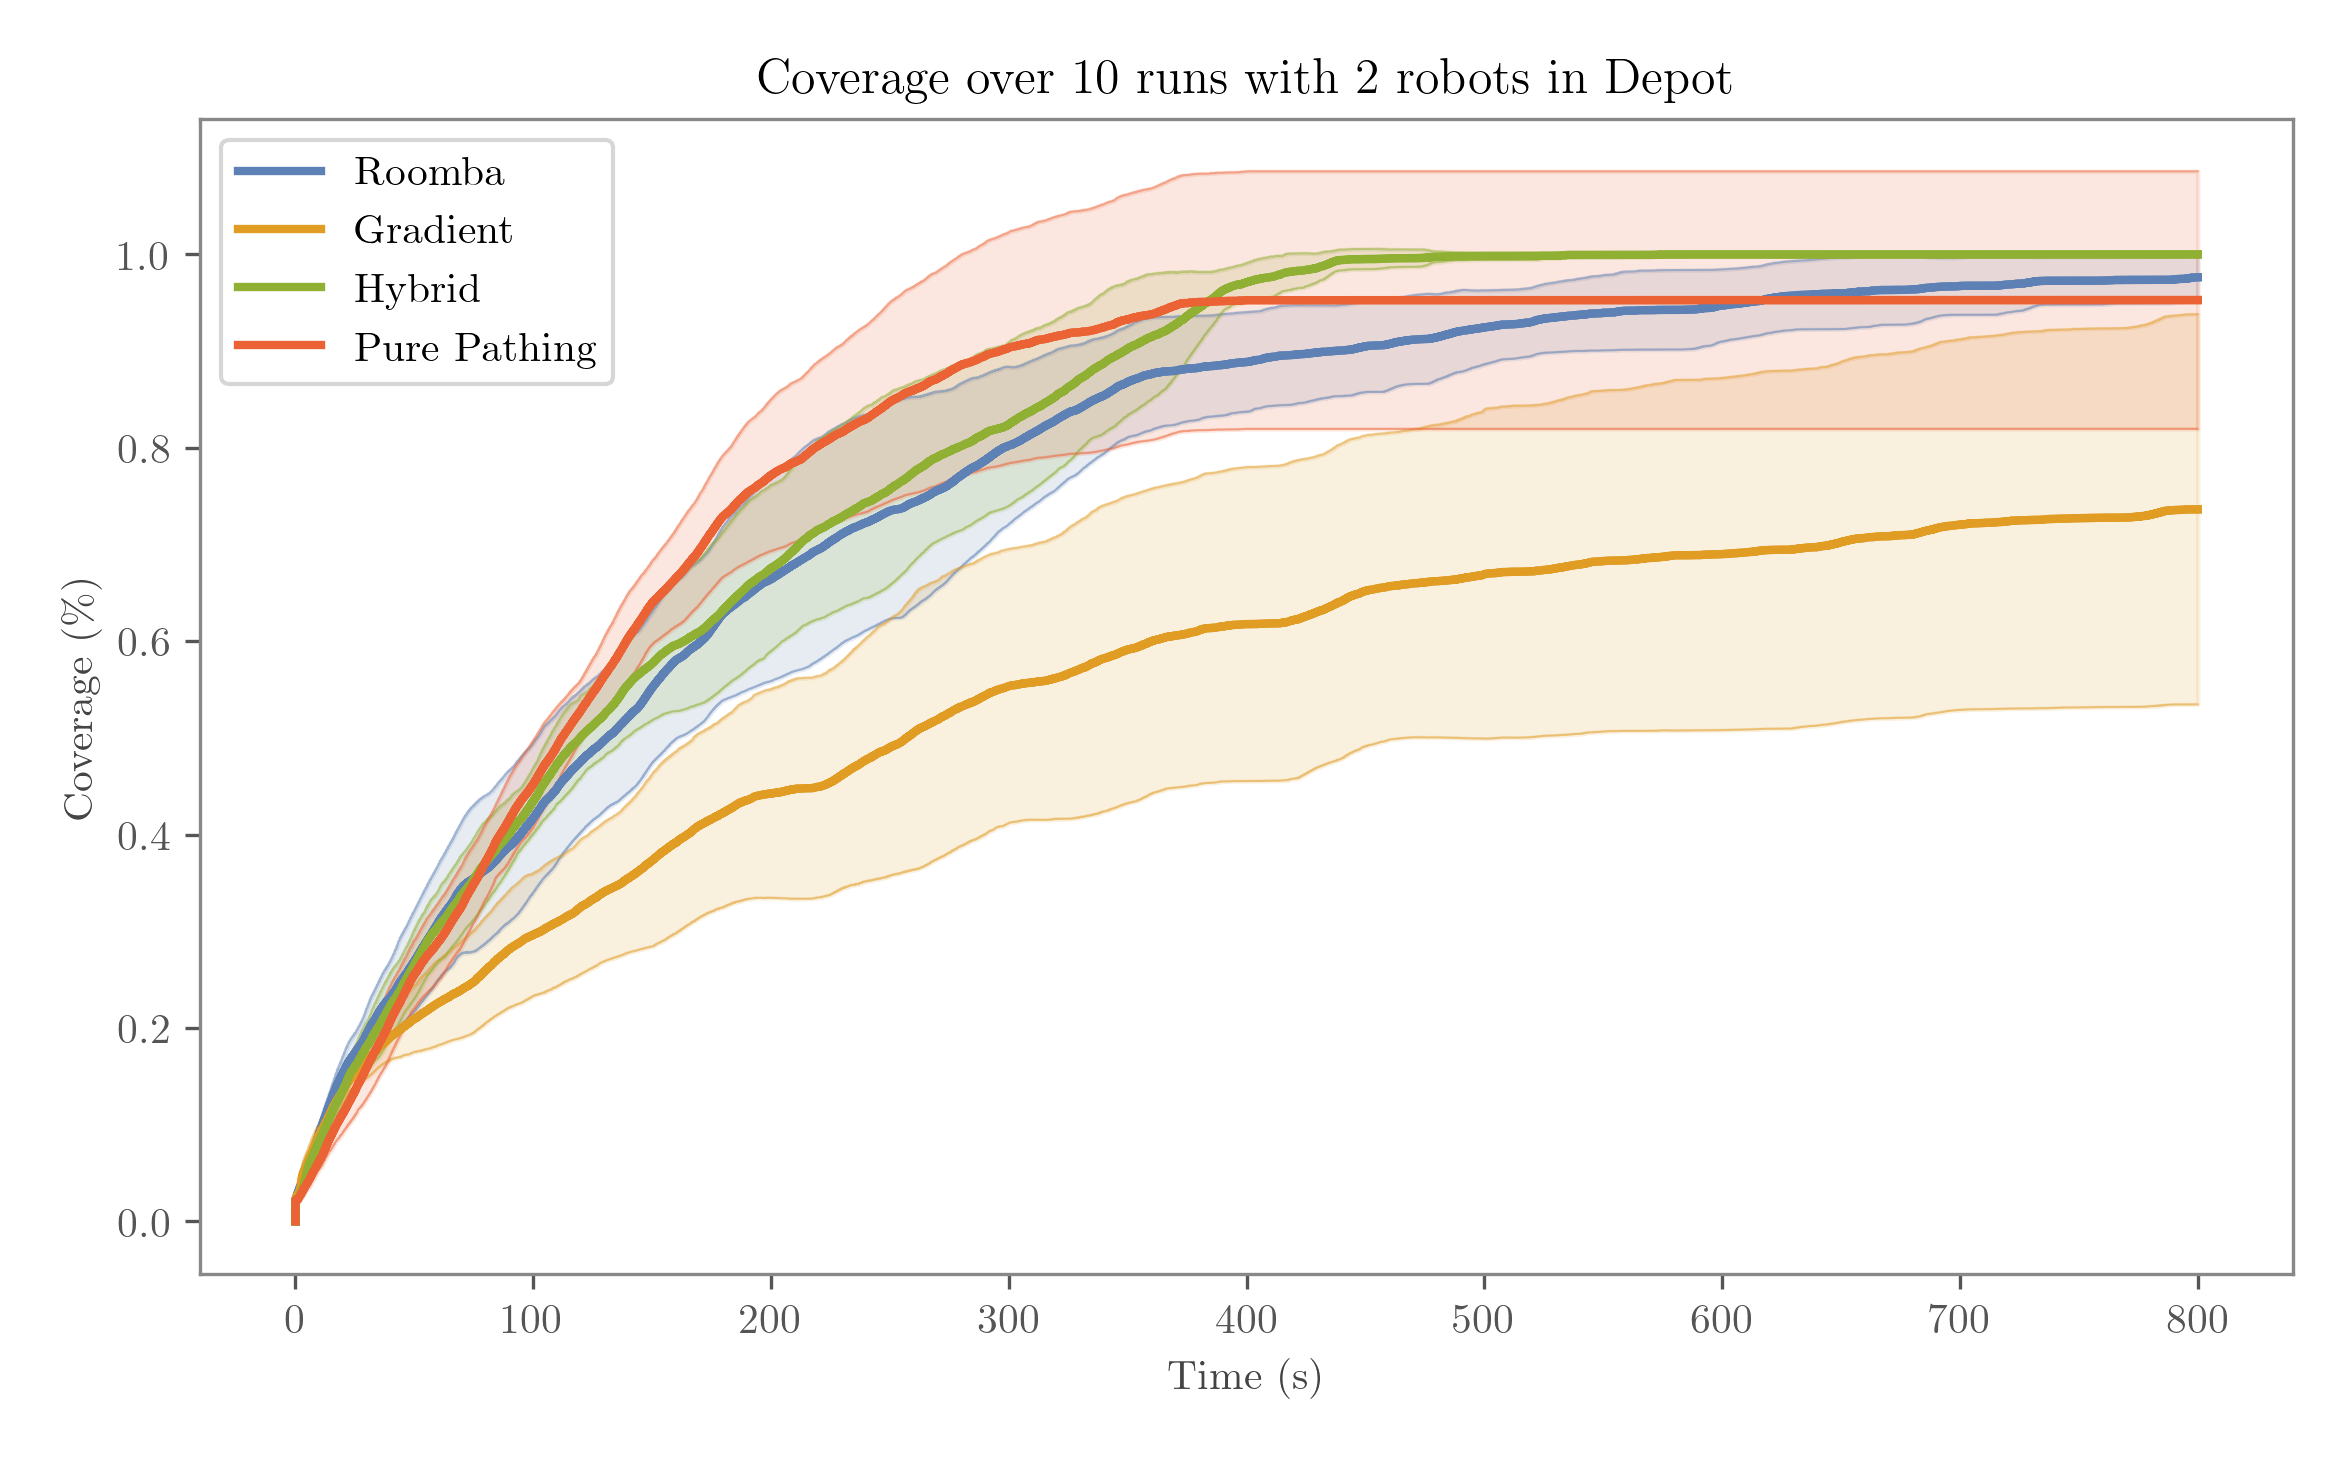
\includegraphics[width=\w]{figures/plots/benchmarks/coverage-over-10-runs-with-2-robots-in-depot.png}
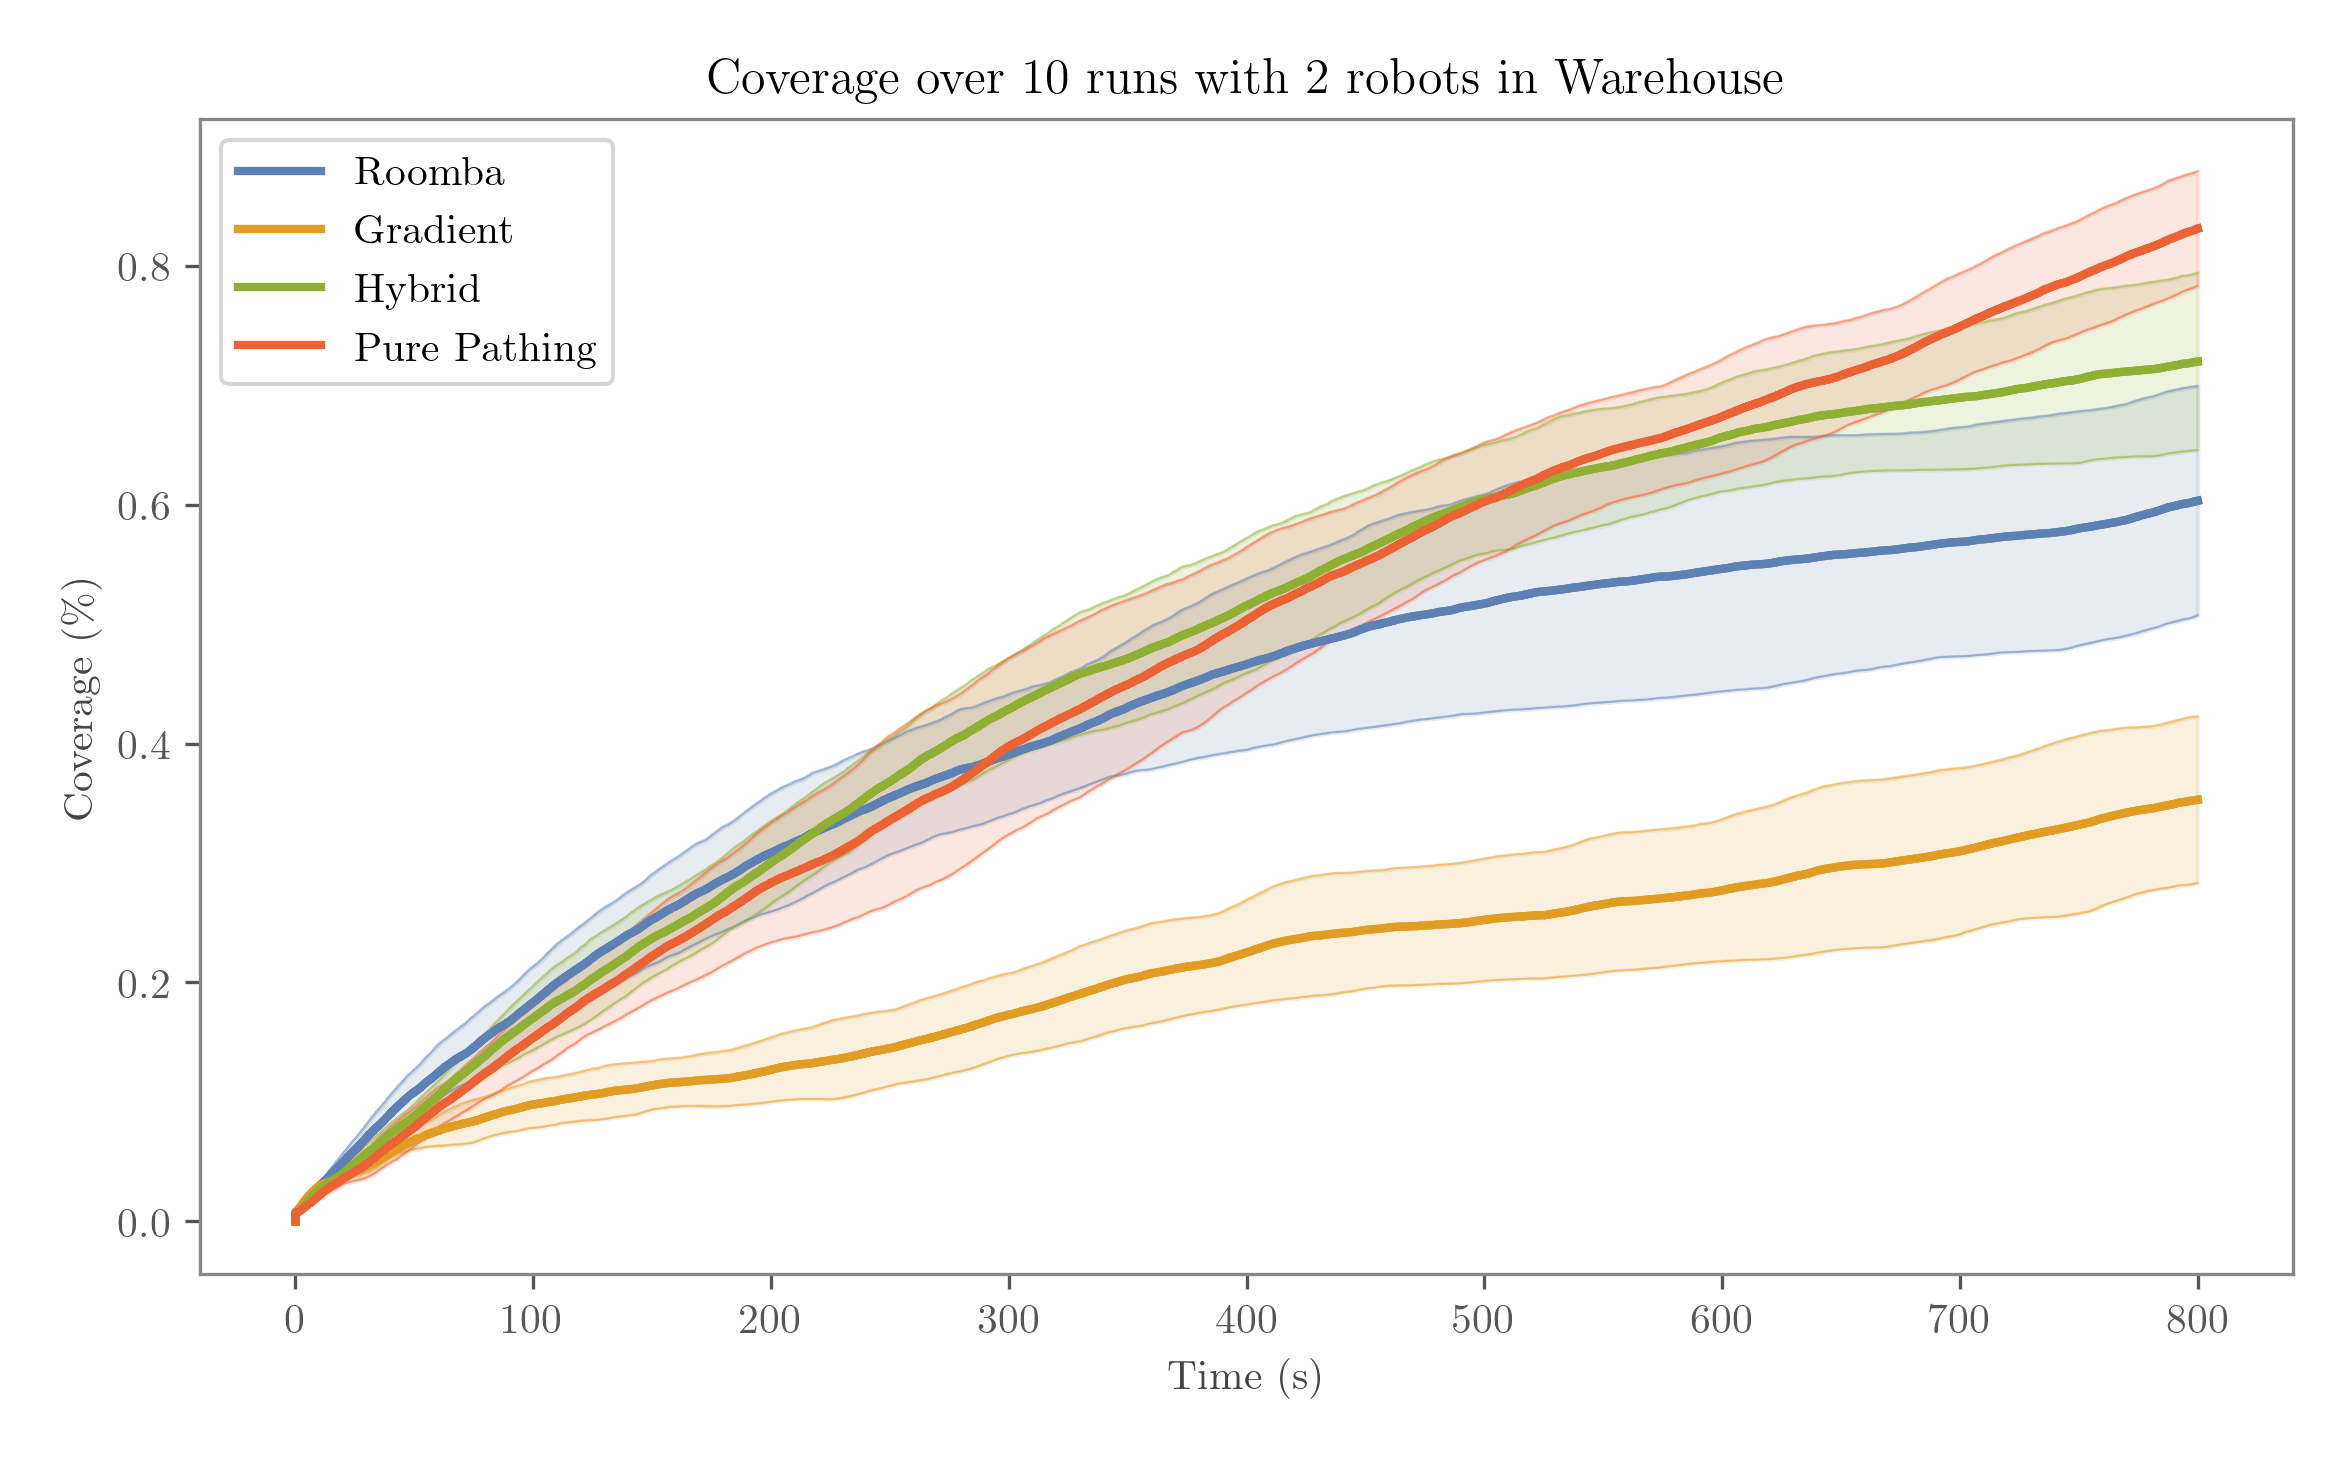
\includegraphics[width=\w]{figures/plots/benchmarks/coverage-over-10-runs-with-2-robots-in-warehouse.png}
\\
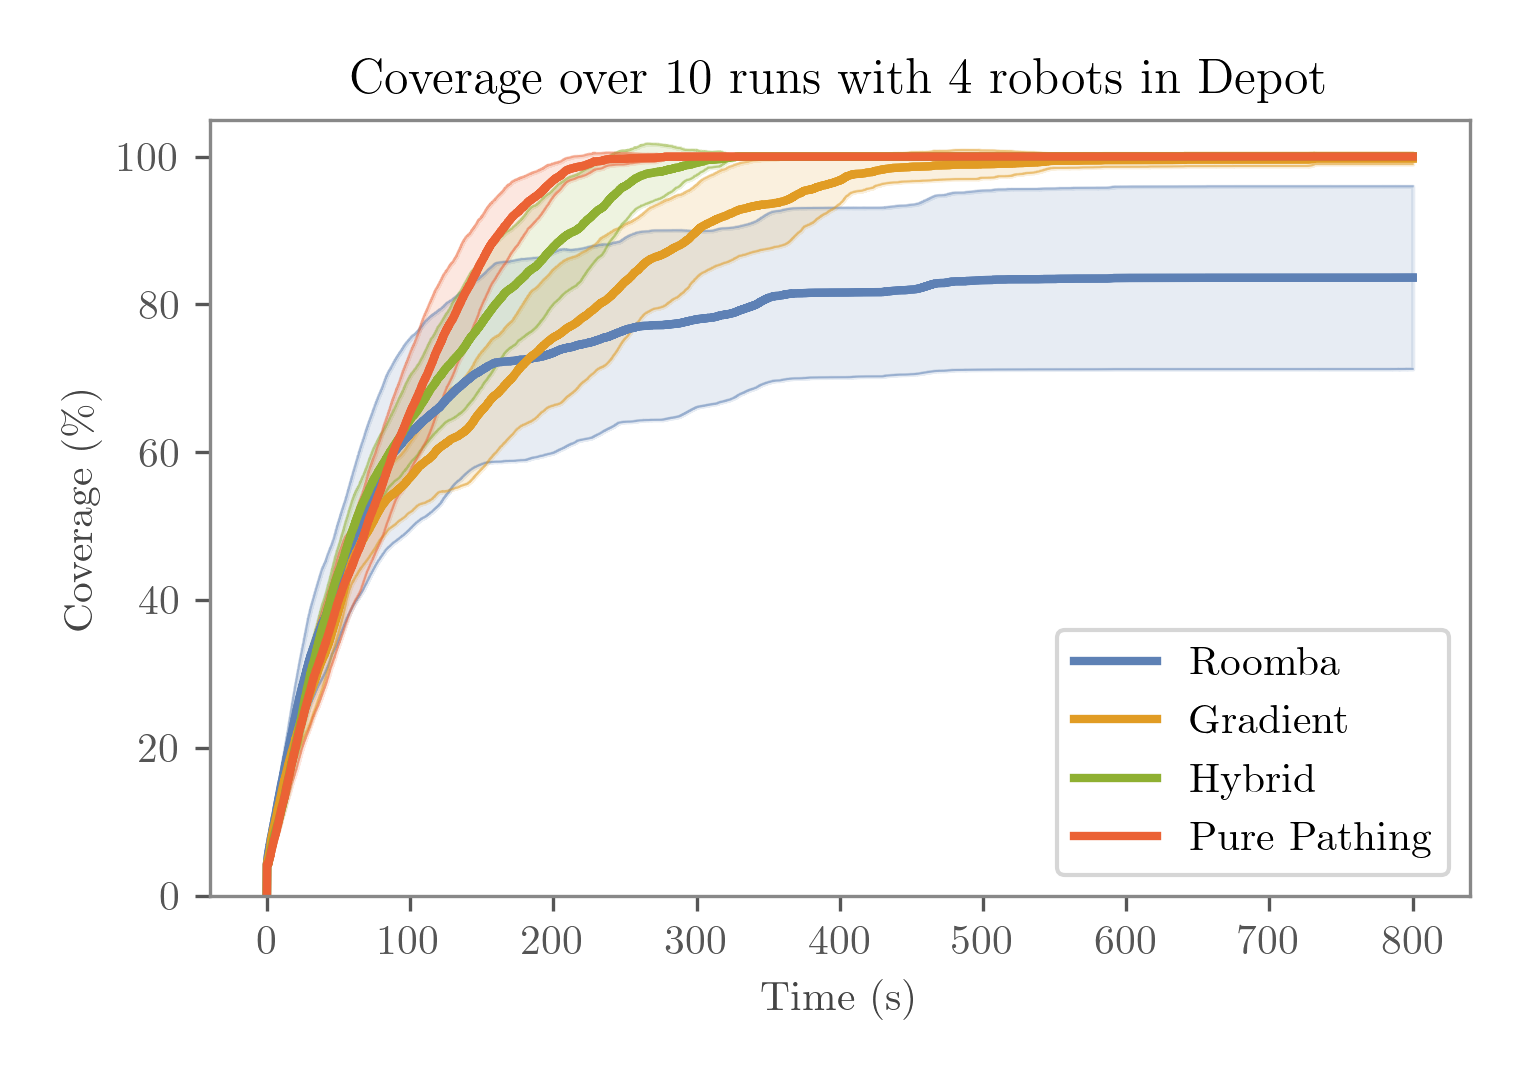
\includegraphics[width=\w]{figures/plots/benchmarks/coverage-over-10-runs-with-4-robots-in-depot.png}
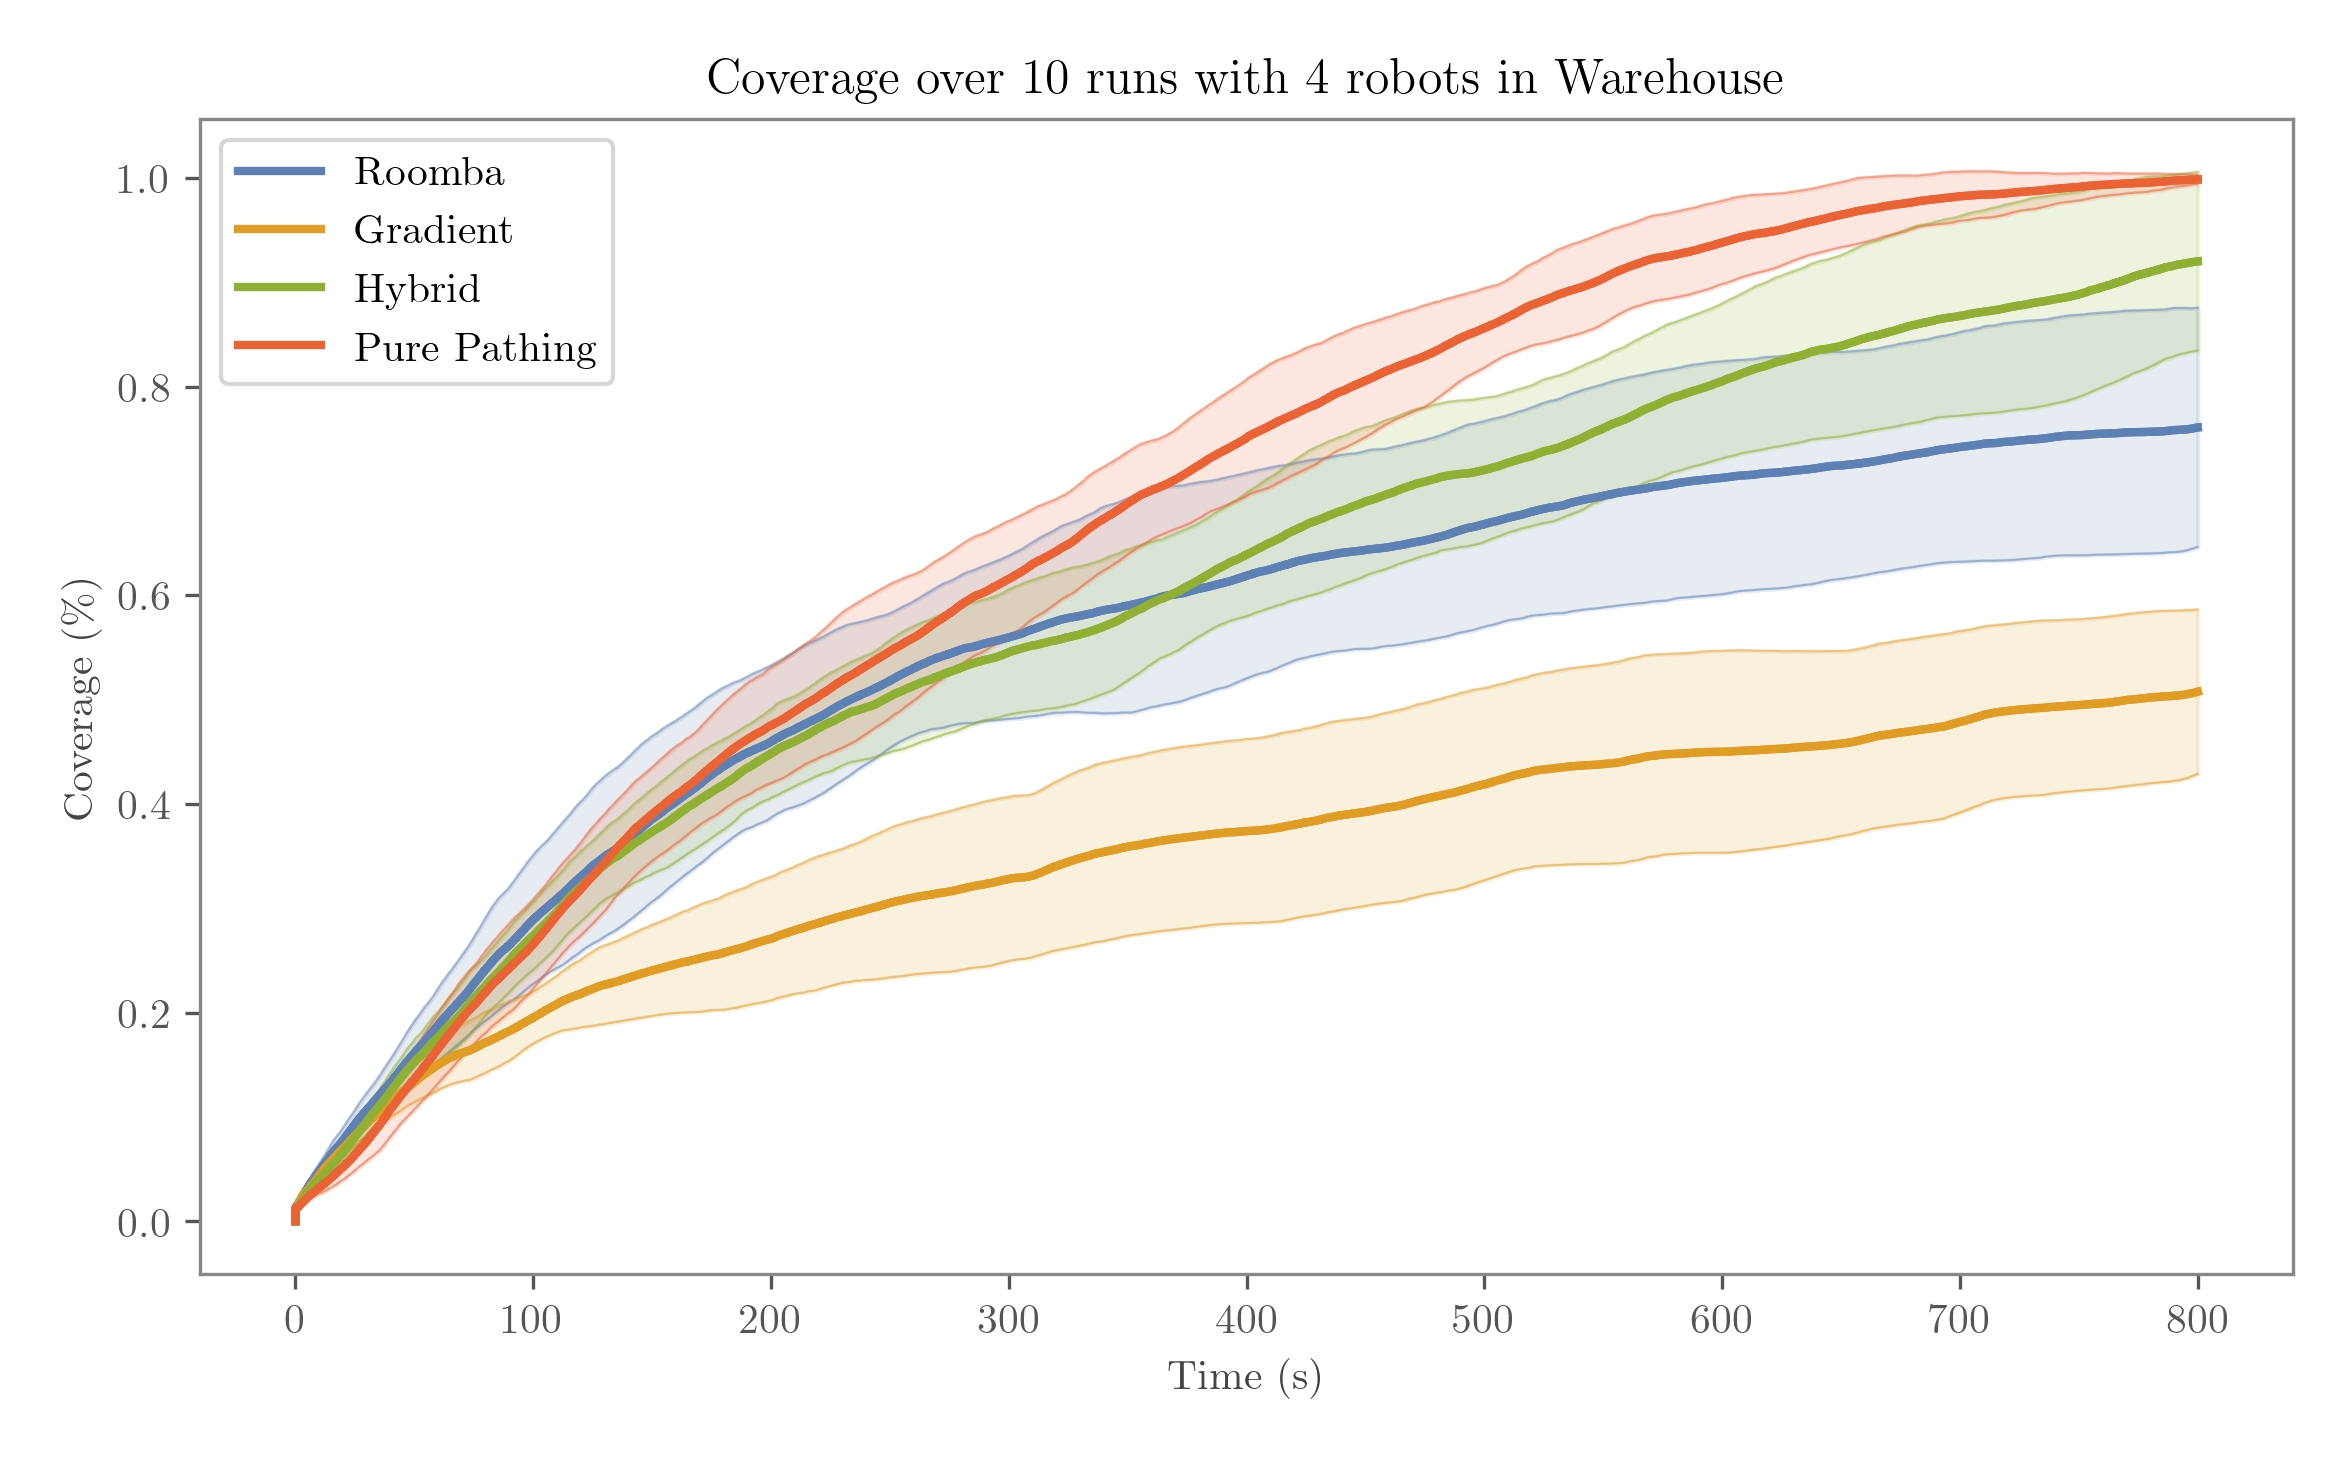
\includegraphics[width=\w]{figures/plots/benchmarks/coverage-over-10-runs-with-4-robots-in-warehouse.png}
\\
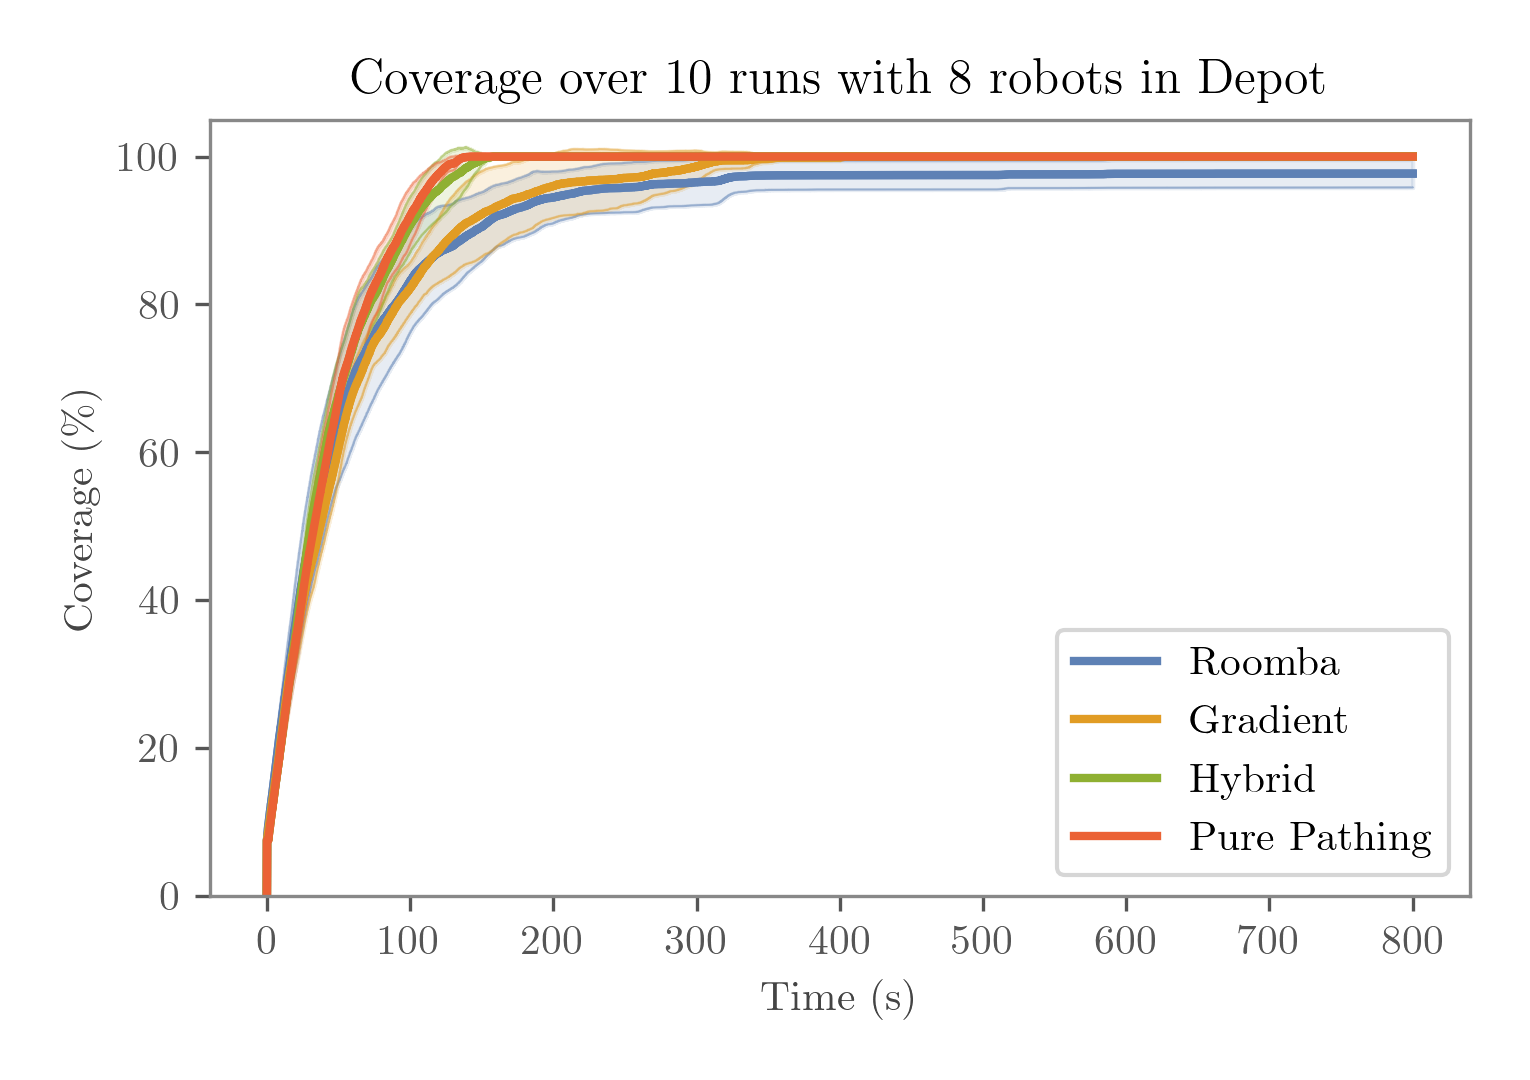
\includegraphics[width=\w]{figures/plots/benchmarks/coverage-over-10-runs-with-8-robots-in-depot.png}
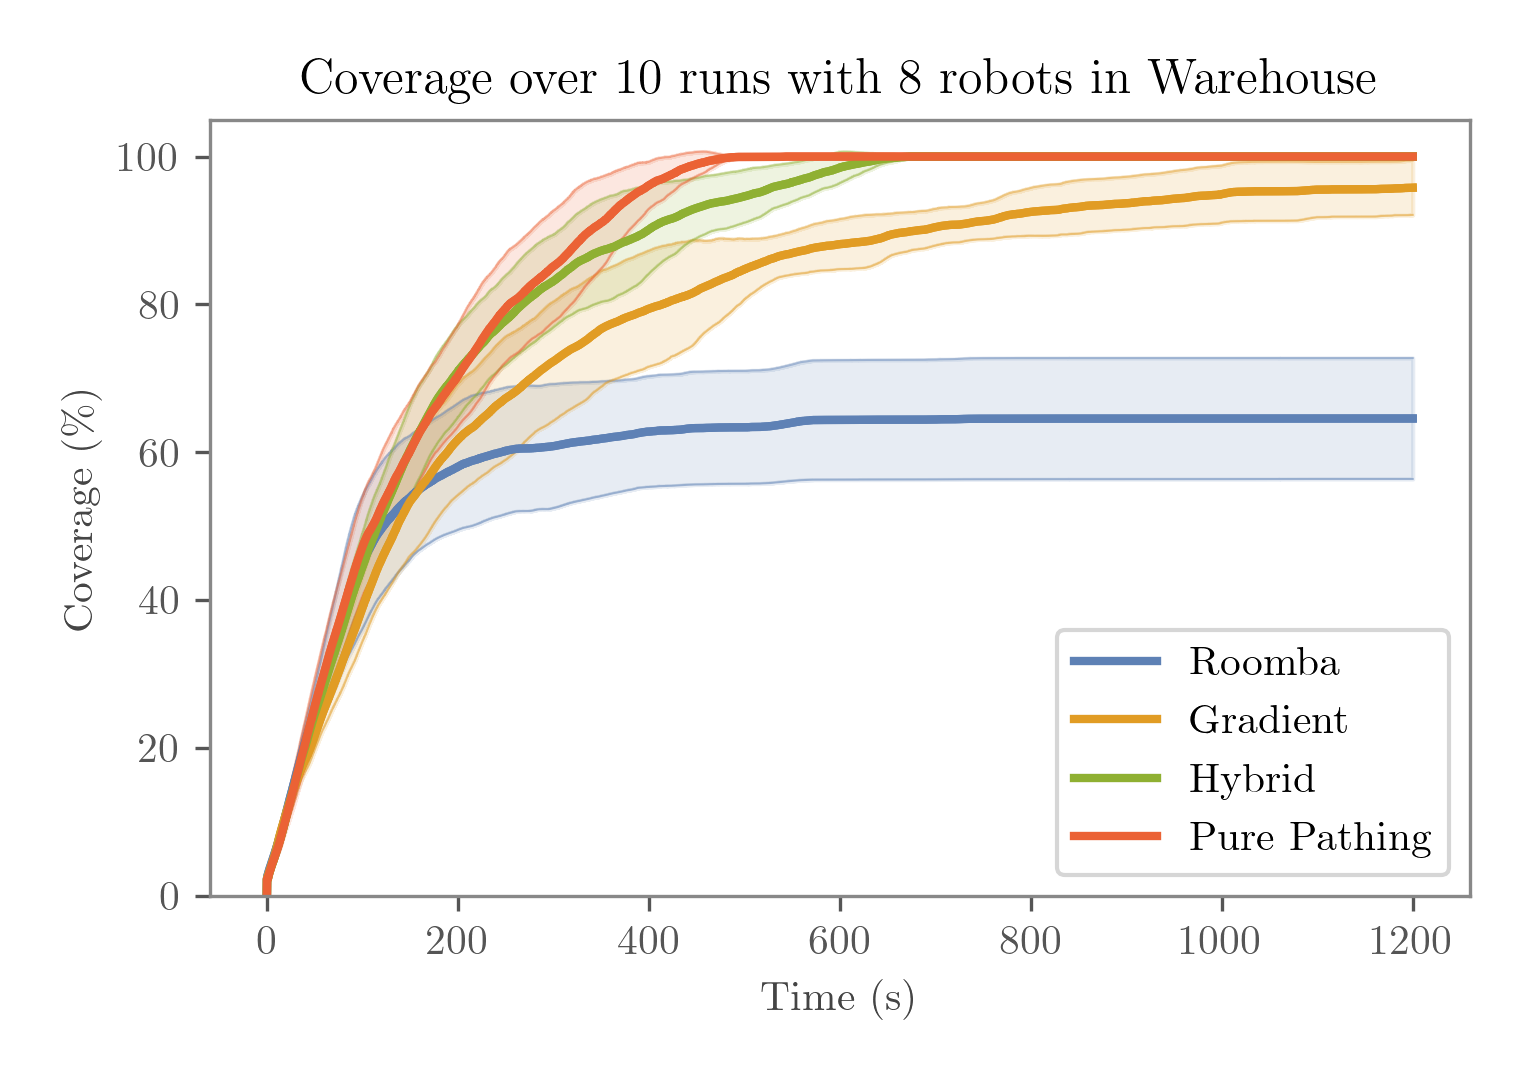
\includegraphics[width=\w]{figures/plots/benchmarks/coverage-over-10-runs-with-8-robots-in-warehouse.png}
\\
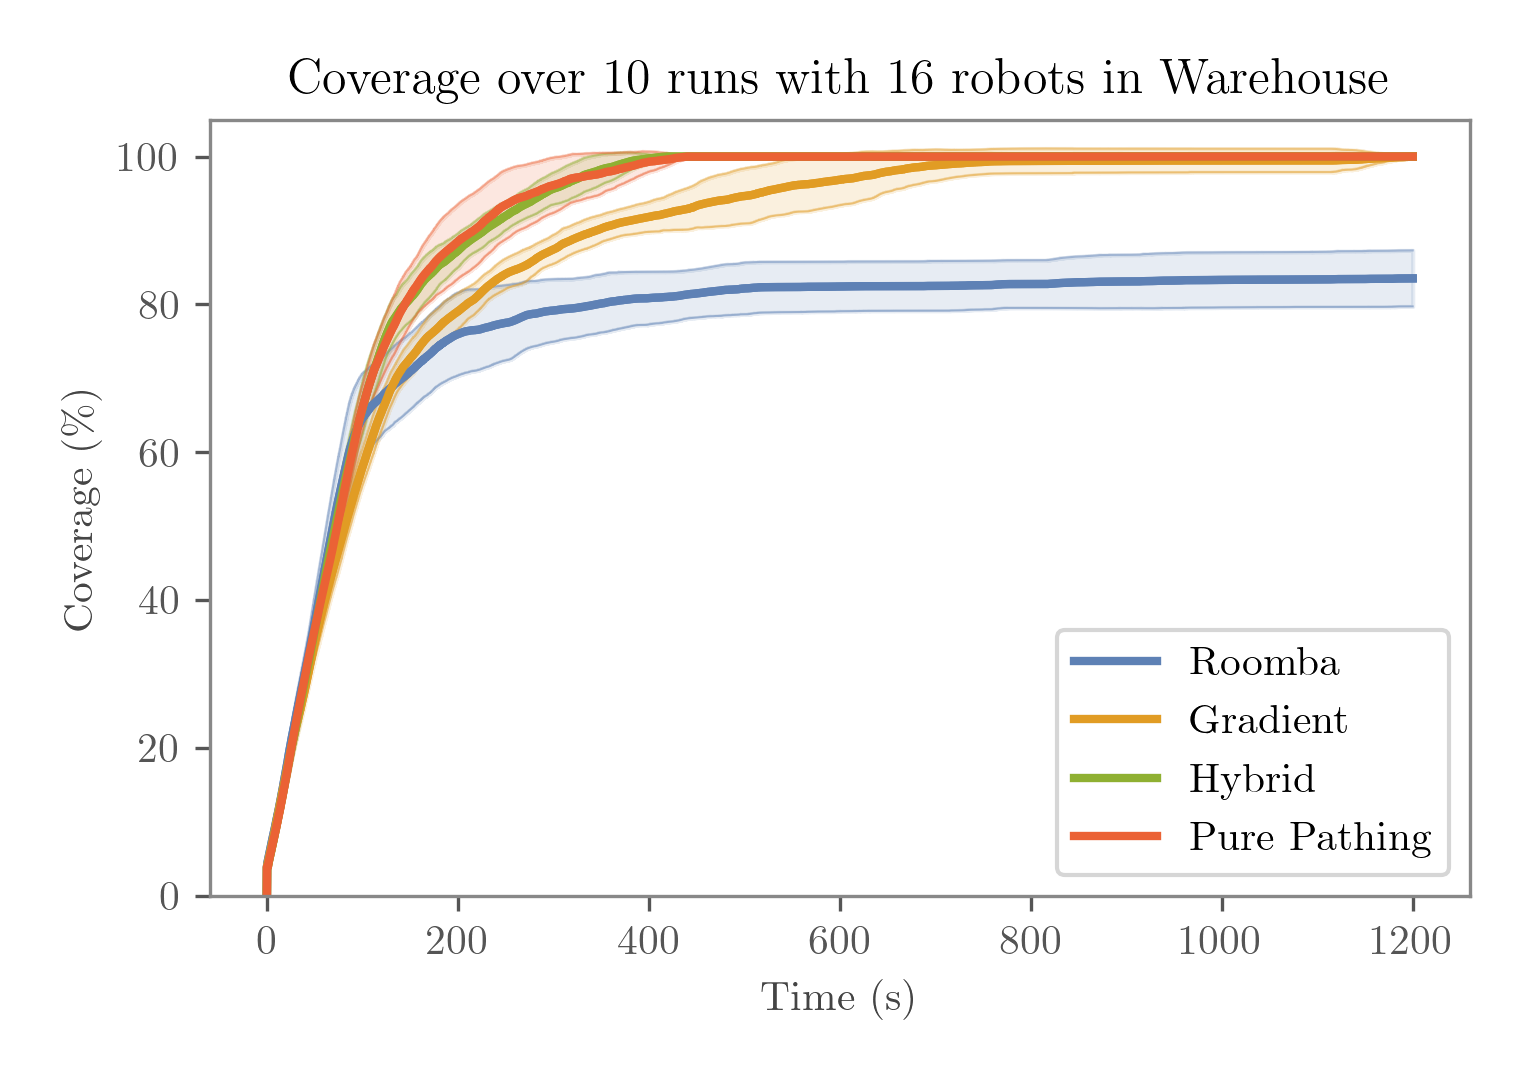
\includegraphics[width=\w]{figures/plots/benchmarks/coverage-over-10-runs-with-16-robots-in-warehouse.png}
